% Dokumentenklasse
\documentclass[a4paper,12pt,liststotoc, parskip=half]{scrreprt}

% ============ Pakete ============
% Dokumentinformationen
\usepackage[
	pdftitle={FM3D Engine},	
	pdfsubject={},
	pdfauthor={Felix Lösing and Max Schmitt},
	pdfkeywords={},
	% Links nicht einrahmen
	% hidelinks
]{hyperref}

% FONTS
\usepackage[utf8]{inputenc}				% UTF-8 Zeichensatz
\usepackage[ngerman]{babel}				% Alle Bezeichnungen auf die deutsche Sprache anpassen
\usepackage[T1]{fontenc}				% Unterstützung für westeuropäische Codierung(Umlaute)


\usepackage{fancyhdr}					% Einfache Bearbeitung von Kopf- und Fußzeile

\usepackage{graphicx}					% Grafiken einbinden
\usepackage{subfig}						% Abbildungen und Tabellen
%\graphicspath{{Anhang/bilder/}}		% Pfad zu Grafiken

\usepackage{lmodern}					% Verändert die Schriftart auf "Latin Modern"
\usepackage{color}						% Farbenmanagement
%\usepackage[printonlyused]{acronym}		% Abkürzungsverzeichnis
\usepackage{booktabs}					% Tabellen ("Publication Quality")
\usepackage[onehalfspacing]{setspace}	% Abstände
\usepackage{geometry}					% Seiten-Layout
\usepackage{authblk}
\usepackage{longtable}
% Zusätzliche Schriftzeichen der American Mathematical Society
\usepackage{amsfonts}
\usepackage{amsmath}

%Package für Todo-Notes
\usepackage{todonotes}

%Erweiterte Referenzen
\usepackage{hyperref}
\usepackage[ngerman, nameinlink, noabbrev]{cleveref}

%Abkürzungsverzeichnis
\usepackage[printonlyused ]{acronym}

% C++ Code Gedöns
\usepackage{listings}
\lstset{numbers=left, numberstyle=\tiny, numbersep=5pt}
\lstset{language=C}

% Zitatgedöns
%\usepackage{multibib}
%\usepackage{hyperref}

%\newcites{Refs,Urls,Graf}{Literaturverzeichnis, Internetadressenverzeichnis, Grafikverzeichnis}

% ============ Kopf- und Fußzeile ============
% Style
\pagestyle{fancy}

% Kopfzeile
\lhead{ }
\chead{ }
\rhead{ }

% Fußzeile
\lfoot{ \leftmark}
\cfoot{\slshape }
\rfoot{\thepage}

% Trennlinien
%\renewcommand{\headrulewidth}{0.0pt}	% keine trennlinie nach der Kopfzeile
\renewcommand{\footrulewidth}{0.2pt}		% Dünne Trennline vor der Fußzeile

% ============ Paketeinstellungen & Sonstiges ============
% Besondere Trennungen
\hyphenation{De-zi-mal-tren-nung}
\hyphenation{Ent-wick-lung}
\hyphenation{ent-wick-eln}
\hyphenation{Library}

%Helvetia FONT
\usepackage{mathptmx}
\usepackage{helvet}

\bibliographystyle{IEEEtran}


% ============ Dokumentbeginn ============

%\setmainfont{Calibri}
\begin{document}
% Seiten ohne Kopf- und Fußzeilen sowie Seitenzahl
\pagestyle{fancy}
%\include{titel}

\title{%
  Programmierung einer Engine für erleichterte 3D-Spiele-Entwicklung \\
  \large ----------------- \\ BG13 \\ ----------------- \\ Groß-Gerau \\ Trebur \\  --------------------------}

\date{\today}
\author{Felix Lösing und Max Schmitt}
\affil{Berufliches Gymnasium Groß-Gerau}

\maketitle
%\newpage\null\thispagestyle{empty}

% Festlegung der Art der Zitierung
%\bibliographystyle{unsrt}
%\bibliographystyle{unsrt}
% Beendet eine Seite und erzwingt auf den nachfolgenden Seiten die Ausgabe aller Gleitobjekte
% (z.B. Abbildungen), die bislang definiert, aber noch nicht ausgegeben wurden. Dieser Befehl fügt,
% falls nötig, eine leere Seite ein, sodaß die nächste Seite nach den Gleitobjekten eine ungerade
% Seitennummer hat. 
\cleardoubleoddpage{}

% Seiten ab jetzt mit Kopf- und Fußzeilen sowie Seitenzahl
\pagestyle{fancy}

% Kopfzeile
\lhead{}
\chead{ \leftmark}
\rhead{}

% Fußzeile
\lfoot{FM3D-Dokumentation}
\cfoot{\thepage}
\rfoot{ %\slshape 
\date{\today} }

% Inhaltsverzeichnis
\begingroup
  \renewcommand*{\chapterpagestyle}{empty}
  \pagestyle{empty}
  \tableofcontents
  %\clearpage
\endgroup

\pagenumbering{Roman}

\begin{acronym}
	\chapter*{Abkürzungsverzeichnis}
	\addcontentsline{SLERP}{chapter}{Abkürzungsverzeichnis}
	\acro{CLR} {Common Language Runtime}
	\acro{CPU} {Central Processing Unit}
	\acro{FBO} {Framebuffer Object}
	\acro{FM3D}{Flying Mind Engine}
	\acro{GPU} {Graphics Processing Unit}
	\acro{IBO} {Index Buffer Object}
	\acro{MVVM}{ModelView ViewModel}
	\acro{PBR} {Physically Based Rendering}
	\acro{VBO} {Vertex Buffer Object}
	\acro{VAO} {Vertex Array Object}
	\acro{WPF}	{Windows Presentation Foundation}
	\acro{XAML}{Extensible Application Markup Language}
	\acro{XML} {Extensible Markup Language}
	\acro{SLERP} {Spherical Linear Interpolation}
\end{acronym}
% Tabellenverzeichnis
\listoftables

% Abbildungsverzeichnis
\listoffigures

\clearpage
\pagenumbering{arabic} 

% Kapitel einbinden

\chapter{Einführung}
\label{c:einführung}
\setcounter{page}{1}
\section[Warum dieses Themenfeld?]{Warum haben wir dieses Themenfeld gewählt?}

Uns ist aufgefallen, dass man bei größeren Schulaufgaben, in denen man auf sich alleine gestellt ist, mehr mit einer Programmiersprache ausprobieren und experimentieren kann. Das Erfolgserlebnis beim Fertigstellen einer Software ist immens. 

Da ein Großteil der Schüler in der heutigen Zeit mit dem Medium „Videospiele“ konfrontiert ist und dieses perfekt zum Ausprobieren ist, kann es für sie ein höchst interessanter Prozess sein, ein eigenes Videospiel zu entwickeln. Dies haben wir auch praktisch in unserem eigenen Unterricht positiv zu spüren bekommen.
Leider ist die Entwicklung eines Spieles ein sehr komplexer Prozess, welcher bei großen Industrien sogar in vier bis fünf Arbeitsbereiche unterteilt wird; (Produzent), Programmierer, Grafiker, Spiele-Designer und Sounddesigner.  \cite{gea}

Für die Entwicklung eines Spieles ist leider einige Fachkompetenz von Nöten, die nicht jeder Schüler besitzt. Zudem ist die Entwicklung „from scratch“ eines Spieles sehr zeitaufwendig und nicht jeder Lehrer kann so viel Zeit für ein Projekt zur Verfügung zu stellen. 
So könnte man nun also eine Engine verwenden, um ein Spiel zu entwickeln. Hier kommt nun aber ein weiteres Problem auf; Die meisten Engines sind sehr kostspielig oder verfügen über eine eigene Programmier-/ Skriptsprache und sind rein zum Spiele-Entwickeln konzipiert, meist auch nur mit kommerzieller Basis, oder um Zeit zu sparen und nicht um die Struktur einer Programmiersprache zu erlernen.

Darum wurde die Flying-Mind 3D [FM3D] Engine entwickelt. Die FM3D Engine besitzt die wichtigsten Komponenten um ein Spiel zu entwickeln;  Ein Mathsystem, ein Memorysystem, ein Filesystem, ein Grafiksystem und einige Funktionen die es sehr leicht machen ein Spiel zu entwickeln.
Zudem wurde ein „Designer“ entwickelt in den man die 3D-Modelle laden, positionieren und die Ausgangssituation des Spiels zu einem Visual-Studio 2015 Projekt konvertieren kann.
Der Lehrer könnte dem Schüler zB. die Aufgabe geben, einen kleinen Roboter durch ein Labyrinth zu einer Fahne hindurch zu manövrieren. Der Schüler kann nun alle Einstellungen im Designer tätigen, sich ein funktionsfähiges Projekt generieren lassen und sich vollkommen auf die Programmierung der Steuerung des 3D-Modell des Roboters fokussieren.

Natürlich können die Schüler mit der Engine auch größere Projekte programmieren und auch für private Projekte gebrauchen. Auch ist die Engine nicht nur für Schüler entwickelt worden. Auch Hobby-Spieleentwickler können mit ihr einfach und simpel eigene Spiele entwickeln, ohne dabei den Überblick im Code zu verlieren.

Die FM3D-Engine kann auch für Programme mit dreidimensionalen Rendering verwendet werden, welche nicht in den Anwendungsbereich Spiele fallen. Darunter fallen zum Beispiel Lehrsoftware, Simulationen oder mehr.

\section{Begriffsdefinitionen}
\subsection{Spiele}	

Bevor man eine Spiele-Engine programmiert, so sollte man sich erst einmal die Frage stellen, was genau ein \textit{Spiel} ist. Wir alle können durch unseren Alltag etwas mit dem Begriff „Spiel“ verbinden, doch müssen wir für allgemeines Verständnis auch hier noch einmal fest definieren, was genau ein Spiel ist;
Brettspiele wie Schach, Dame, Mühle; Glücksspiele wie Poker, Roulette, Lotto; Kinderspiele wie Topfschlagen; und natürlich die Video-Spiele; Dies sind für uns alle Spiele, doch warum?
Schlägt man den Begriff „Spiele“ in dem Buch „Der Brockhaus“ nach, so bekommt man die folgende Definition:

\begin{quote}
	„Spiel das, 1) jede Tätigkeit, die aus Freude an dieser selbst geschieht, im Ggs. zur zweckbestimmten Arbeit. […]“ (Aus \cite{brockhaus})
\end{quote}

Spiele dienen also der Unterhaltung und dem Zeitvertreib des Spielers.
Diese Beschreibung trifft auch auf Videospiele zu, denn auch Videospiele sind größtenteils nicht zweckbestimmt und dienen nur zur Unterhaltung des Spielers.
In dem Buch „Game Engine Architecture“ \cite{gea} ist ein Verweis auf das Buch „A Theory
of Fun for Game Design“ in dem Raph Koster den Begriff „Spiel“ wie folgt definiert:

\begin{quote}
	„Ein Spiel ist eine interaktive Erfahrung, die dem Spieler ermöglicht, steigende Herausforderungen von Mustern, welche der Spieler im Laufe des Spieles lernt, zu meistern.“
	(Aus \cite{theoryoffun}, Zitat aus dem Englischen übersetzt)
\end{quote}
\subsection{Video-Spiele}

In der Videospielindustrie ist ein Spiel eine Software, die Bilder oder virtuelle dreidimensionale Objekte, die durch Spieler-Eingaben beeinflusst werden können, um ein vom Entwickler (oder genauer vom Spieldesigner) festgelegtes Ziel zu erreichen. 
Im Normalfall wird vom Spieler ein menschen- oder tierähnliches Wesen oder Fahrzeug durch ein Eingabegerät fortbewegt. Betont wird hier der Normalfall, da es verschiedene Genres oder Videospiel-Formen gibt. Hier ist die Kreativität des Entwicklers gefragt.

Gregory definiert in dem Buch „Game Engine Architecture“ ein Video-Spiel aus technischer Sicht als „soft real-time interactive agent-based computer simulations“ \cite{gea} (interaktive agentbasierte computergestützte Echtzeitsimulationen).
Doch wie kommt man zu diesem Begriff?

Die meisten Spiele bilden eine Simulation einer realen oder fiktiven Welt ab, die mathematisch modelliert wird. In einer Agent basierten Simulation interagieren verschiedene „Entities“ miteinander, weshalb auch objektorientierte Programmiersprachen (wie z.B. C++ oder Java) verwendet werden.
Solche interaktiven Videospiele sind zeitlich abhängige Simulationen, da sich Eigenschaften, wie zum Beispiel das Aussehen, in dieser fiktiven Welt mit der Zeit verändern. Außerdem sollte das Programm in Echtzeit auf die Eingaben des Spielers reagieren.

\subsection{Game-Engine}	
\label{engine}
Wenn man Spiele entwickeln möchte, so taucht früher oder später das Wort „Game-Engine“ auf. Einige Entwicklungsfirmen verweisen auch auf ihre Engine, um technisch besser da zu stehen und ihrem Spiel ein besseres Ansehen zu verschaffen. Heißt das aber, mit einer besseren Game-Engine kann man ein besseres Spiel entwickeln? Um dies heraus zu finden, sollte man sich erst einmal anschauen, wie solche Engines funktionieren und aufgebaut sind.

Frühere Spiele wie „Tetris“, „PacMan“ oder „Space-Invaders“ wurden immer „from scratch“  entwickelt. Die Entwickler besaßen also so gut wie gar kein Gerüst, bevor sie dieses Spiel programmierten. Da die meisten Spiele aber einen ähnlichen Aufbau besitzen, fiel auf, dass man immer einen ähnlichen Programm-Code verwenden könnte, um die Grundstruktur eines Spieles zu entwickeln. Vereinfacht verfügt ein Spiel über die Zentralbereiche der Grafik und die der Logik. Die Soundausgabe ist bei Spielen optional, da auch Spiele ohne Musik und Sound-Effekte existieren. Dennoch bieten die meisten Engines auch hierfür ein Grundgerüst.

Eine Game-Engine bietet dem Entwickler also diese Rahmenfunktionen, die seiner Software das Grundgerüst liefert. Dies heißt in der Softwareentwicklung „Framework“. 
Moderne Game-Engines sind heutzutage auf ein bestimmtes Genre oder auf bestimmte Aufgabenbereiche spezialisiert. So gibt es Game-Engines sowohl für 2D- als auch 3D-Spiele. Der „GameMaker“ von „YoyoGames“ ist zum Beispiel auf 2D-Spiele spezialisiert. Doch kann man auch Spiele in 3D mit ihm erstellen. Die „CryEngine“ hingegen ist hauptsächlich für 3D-Spiele konzipiert. (Für weitere Details zu diesem Thema siehe \ref{engines}.)


\section{Geschichte}
\subsection{Vergangenheit bis heute}
\label{vergangenheit}
Die ersten Konsolen auf dem Markt besaßen geringen Speicher. So mussten die Entwickler die Spiele immer speicherkalkuliert entwickeln, sodass sie möglichst klein und speichersparend waren. Da man also für jedes Spiel einen optimierten Code benötigte, waren Game-Engines von Drittanbietern nicht nötig.

Erst mit den 3D-Spielen und verbesserter Hardware wurden die Game-Engines von externen Unternehmen populär. Konsolen und PCs verfügten nun über genug Speicher und man musste nicht mehr auf jedes Byte achten. Die "`Angst"', man könne Speicher verschwenden oder ein zu großes Programm entwickeln, wurde mit der Zeit immer mehr zurück gedrängt.
Da die Entwickler nun auch Spiele herausbringen wollten, welche auf dem Markt besser ankommen und technisch fortschrittlicher sind, wurde der Code der Software um vieles komplexer.\todo{!}

So kam man schnell auf die Idee, ein System zu entwickeln, das für die Hauptbereiche eines Spiels ein Grundgerüst baut, die Software in Betrieb hält und das immer wieder verwendbar ist. Mit einer Game-Engine konnte man nun Zeit und Aufwand beim Programmieren sparen, mehr Zeit in die Optimierung des Spieles stecken und sich mehr Zeit für die Spielinhalte nehmen. 

\input{01einfuhrung/Zukunft}

\section{Engines}
\label{engines}
\subsection{GameMaker - YoyoGames}

Die zuerst für 2D-Animationen konzipierte Game-Engine "'GameMaker"` (In den Anfängen \textit{Animo}) wurde von Overmars erstmals im Jahre 1999 veröffentlicht und ist nun als "'GameMaker:Studio"` bekannt. Zunächst hat man sich bei der Entwicklung sehr stark auf die 2D-Spiele Entwicklung konzentriert. Mittlerweile kann man mit ihr sogar 3D-Spiele entwickeln. 

Das Programm ist momentan in drei verschiedenen Versionen erhältlich (Stand 2017). Darunter auch eine kostenlose Version mit beschränkten Funktionen.
Die Benutzeroberfläche ist sehr simpel gehalten und ist so konzipiert, dass sogar ein Leihe den Programmablauf eines Spieles durch einfaches "Drag'n'Drop" von Schaltflächen schnell erstellen und strukturieren kann. Zudem besitzt der "'GameMaker"` eine eigene Skript-Sprache, welche einige der höheren Programmiersprachen als Vorbild nimmt.

Die mit der GameMaker-Engine entwickelten Spiele werden mit verschiedene \textit{Resourcen} entwickelt;
Sprites, Sounds, Backgrounds, Paths, Scripts, Fonts, Timelines, Objects und Rooms. 
Auch wir wollten dies so ähnlich in unserem Designer handhaben und haben uns von dem Prinzip der Resourcen inspirieren lassen. \ref{designer}

Die Spiele können für diverse gängigen Betriebssysteme (Windows, Android, iOS ua.) aber auch für populäre Spielekonsolen (PlayStation, XBox ua.) kompiliert werden. 

\subsection{Unity3D - Unity Technologies}

"`Unity3D"' ist eine Game-Engine der Firma \textit{Unity Technologies}, welche erstmals im Jahre 2005 veröffentlicht wurde. Sie ist für die 3D-Spiele Entwicklung konzipiert, besitzt eine eigene 2D-Engine, ist weitaus komplexer als der "`GameMaker"' und bietet somit auch mehr Funktionen. 
Mit ihr kann man Spiele für Computer, aber auch Spielkonsolen, mobile Geräte und Webbrowser entwickeln. Sie ist für Windows, Linux (nur Beta) und OSX in vier verschiedenen Versionen erhältlich, unter denen sich auch eine kostenlose Version befindet. Das Programm beinhaltet zudem noch einen 3D-Terrain-Modellierer, Baum- und Pflanzen-Modell-Editor, Werkzeuge für Partikeleffekte und ein Tool für Bewegungssteuerung für Charaktere.

Die grafische Entwicklungsumgebung ähnelt sehr modernen 3D-Animationsprogrammen. Sie stellt im Hauptfenster eine Spiel-Szene dar und verfügt zudem über eine sogenannte \textit{Timeline}, in der der Zeitablauf des Spieles dargestellt wird. In Menüs kann man Parameter des Spieles verändern und sie für die Strukturierung des Spieles verwenden. 

Das Spiel-Scripting basiert auf dem \textit{Mono}-Compiler und bietet verschiedene Scriptsprachen, darunter auch C\# und eine vom Entwicklerteam eigens entwickelte Sprache "`UnityScript"'. Sie ist hauptsächlich für \textit{Cross-Platform} Programme gedacht. Das heißt, dass alle Scripte sofort für verschiedene Geräte exportiert werden können, ohne davor den Code an das Gerät anpassen zu müssen.

Eine aktuelle Szene besteht aus \textit{Game-Objects}, denen man verschiedene Eigenschaften (Materialien, Klänge, physikalische Eigenschaften, Skripte) zuordnen kann. Dies haben wir auch bei unserem Designer mittels Komponenten realisiert (siehe \cref{designer} oder \cref{entitysystem}).

Aufgrund dieser Komplexität ist die "`Unity3D-Engine"' eher für Fortgeschrittene geeignet und braucht weitaus mehr Einarbeitungszeit als der "`GameMaker"', sie bietet jedoch auch mehr Möglichkeiten.
Bei der Auswahl einer geeigneten Engine muss man abwägen, ob eine einfach zu bedienende Engine auch allen erforderlichen Entwicklungsmöglichkeiten bietet.


\chapter{Theorie}
\label{theorie}

\section[Rendering]{Rendering\cite{GLReference, OglDev, ThinMatrix, SparkyEngine, GLTut}}
\label{rendering}
\subsection{OpenGL Grundlagen}

Die FM3D-Engine verwendet für die Darstellung von 3D-Szenen die Grafikbibliothek OpenGL. (Genaueres zu der Bibliothek erfährt man in \cref{opengl}). Mit OpenGL ist es möglich verschiedene kleine grafische Objekte zu rendern. Dieses entsprechen drei geometrischen Grundobjekte (\textit{Primitives}): Punkte, Linien und Dreiecke. Zudem gibt es verschiedene Möglichkeiten diese aneinander zu reihen, wie in \cref{OpenGLPrimitives} dargestellt ist. Sie können alle einzeln, aber auch aneinanderhängend gerendert werden, sodass Speicher bei den angrenzenden Eckpunkten gespart wird. Diese \textit{Primitives} werden durch ihre Eckpunkte oder auch \textit{Vertices} definiert. Diese beschreiben eine Position in einen dreidimensionalen Raum. OpenGL arbeitet mit einem orthografischem Koordinatensystem. Das heißt: Alle drei Achsen sind orthogonal zu einander und reichen von -1 bis 1.

\subsubsection{Frame buffer}
Das aktuelle Bild wird in mehreren Buffern gespeichert. Die Größe der Buffer ist direkt proportional zu der Pixelanzahl des \textit{Viewports}, also zu dem Bereich in welchem das gerenderte Bild dargestellt wird. Am wichtigsten ist der Color-Buffer. Dieser speichert die Farbe jedes Pixels in vier Floats. Jeweils einen für Rot, Grün, Blau und einen Alpha-Wert, welcher die Transparenz beschreibt. Des Weiteren gibt es den Depth-Buffer. Dieser ist selten auch als Z-Buffer in der Literatur zu finden. Er beschreibt den Abstand zwischen dem aktuell gerenderten Pixel und der Kameraebene. Diese Information wird als Farbinformation in dem Depth-Buffer gespeichert. 
Man benötigt nur einen Channel\todo{welcher Channel?}, da nur ein einziger Zahlenwert gespeichert werden muss. So ist, wenn man den Buffer anzeigt nur ein Schwarz-Weiß-Bild zu sehen. Je heller der Pixel ist, desto weiter weg befindet er sich. Die Größe des Depth-Buffer ist einstellbar. Je größer er ist, desto größer ist auch die Präzision, wobei der Depth-Buffer immer eine viel größere Präzision in der Nähe der Kamera besitzt und nach weiter hinten an Präzision verliert. Dies ist von Vorteil wenn Objekte sehr nah an der Kamera gerendert werden, da dort eine sehr hohe Präzision erforderlich ist. Weit weg von der Kamera ist die Präzision aber nicht sehr relevant. Der Depth-Buffer ist optional. Wird er nicht verwendet, so kann nicht die räumliche Anordnung der Primitives ermittelt werden. Welcher Pixel am Ende angezeigt wird, ist von der Reihenfolge, in der die Primitives gerendert werden, abhängig, wobei das zuletzt gerenderte Primitve ganz vorne zu sehen ist. Diese Buffer sind in \cref{DepthBuffer} dargestellt. 

Zudem gibt es noch den \textit{Stencil-Buffer}. Dieser ist auch optional und ordnet jedem Pixel einen bestimmten Wert zu. Er kann verwendet werden, um bei bestimmten Pixeln das Rendern zu verhindern, wie er dies umsetzt ist einstellbar. Es ist möglich verschiedene Operationen durchzuführen, wenn ein Pixel gerendert wird. Es ist zum Beispiel möglich, dass der Stencil-Wert auf 1 gesetzt oder er um 1 erhöht wird. Zudem ist es möglich den Stencil-Test einzustellen. Dieser wird bei jedem Renderprozess eines Pixels ausgeführt. So kann man zum Beispiel erreichen, dass nur dort, wo der Stencil-Buffer den Wert 1 besitzt ein Pixel gerendert wird. Dadurch können \textit{Schablonen} erstellt werden, bei welchen Objekte gerendert und bei welchen nicht gerendert werden können. daher auch der Name. \todo{Stencil buffer?} 
Alle Buffer zusammen werden in einem \ac{FBO} gespeichert. Dieses ermöglicht das gleichzeitige aktivieren aller zugehörigen Buffer, sowie das Anzeigen des Color-Buffers auf dem Bildschirm. Es muss nicht speziell ein \ac{FBO} erstellt werden. Wenn keines erstellt wird, so wird standardmäßig direkt auf den \textit{Screen-Buffer} gerendert. Ein weiterer Vorteil ist, dass man ein \ac{FBO} sowohl als Output (die häufigere Verwendung) als auch als Input verwenden kann, so kann man zum Beispiel eine gerenderte 3D-Szene in einer anderen 3D- oder 2D-Szene einfügen.  

\subsubsection{Buffer Objects}
Will man einen oder mehrere dieser \textit{Primitives} rendern, so laufen die Daten, welche diese \textit{Primitives} definieren, durch verschiedene Schritte. Diese werden in der Literatur auch oft allgemein als die Rendering-Pipeline bezeichnet. Bei Verwendung dieser Pipeline können immer nur eine Art von Primitives gleichzeitig gerendert werden können.
Die Daten werden dabei als Buffer auf der \ac{GPU} gespeichert, verwendet werden dazu die \acp{VBO}, welche als Byte-Arrays vorliegen. Bei ihnen muss manuell eingestellt werden, wie diese Bytes interpretiert werden sollen. Dafür beschreibt man verschiedene Attribute mit Byte-Anzahl und Größe sowie DatenTyp. Zum Beispiel beschreiben die ersten 4 Bytes einen Float und die darauffolgenden 12 einen 3D-Float-Vektor. Es können auch mehrere \ac{VBO}s zusammengefasst werden in einen \ac{VAO}. \acp{VAO} speichern zusätzlich den Zustand der enthaltenen \acp{VBO} und die Information welche Attribute verwendet werden. Zusätzlich zu einem oder mehreren \acp{VBO}, kann ein \ac{IBO} verwendet werden. Dieser besteht aus einem Array von Ganzzahlen und wird ebenfalls auf der \ac{GPU} gespeichert. Er beschreibt welche Vertices für welche Primitives verwendet werden sollen, wo bei Vertices mehrfach verwendet werden können. Der Index-Buffer wird nacheinander durchgegangen und jeder darin gespeicherte Index steht für einen Wert im \ac{VBO}. Wenn man also viele Primitives hat, die sich einen gemeinsamen Punkt teilen, ist es effizienter einen Index-Buffer zu verwenden, da dieser geimeinsame Vertex nur einmal gepseichert werden muss und in der Regel ist die Größe eines Vertex weitaus größer als die Größe eines Index. Zum Beispiel können mit dem \ac{IBO} { 0, 1, 2, 2, 1, 3} zwei Dreiecke gerendert werden, es werden aber nur 4 Vertices benötig (0-3).\cite{ThinMatrix}

\subsubsection{Pipeline\cite{Pipeline}}
Ein \ac{VBO} oder ein \ac{VAO} entsprechen dem Input der Pipeline, wobei in modernen Programmen immer \acp{VAO} verwendet werden, da sie zusätzliche Informationen speichern können.

In der Pipeline bestehen mehrere Schritte aus Shadern. Dies sind kleinere Programme, welche auf der Grafikkarte ausgeführt werden. Sie werden in der Programmiersprache GLSL programmiert. Dies eine spezielle Sprache, die für Shader von OpenGL verwendet wird. Sie ähnelt stark C und besitzt einige bereits zur Verfügung gestellte Funktionen um linear algebraische Rechnungen durchzuführen. Sie unterscheidet sich stark zwischen den einzelnen OpenGL Versionen, da ständig neue Features hinzugefügt werden. Die FM3D-Engine besitzt daher auch teilweise für verschiedene OpenGL-Versionen verschiedene Shaderimplementationen.

Ein grober Überblick über die Rendering Pipeline wird in \cref{RenderingPipeling} gegeben. Der erste Schritt ist das Erstellen der Daten und das Angeben der Attribute, wie vorher beschrieben. Diese sind dann der Input für den \textit{Vertex-Shader}. 

Im \textit{Vertex-Shader} werden die Positionen einzelner Vertices festgelegt, daher wird er für jeden \textit{Vertex} einmal ausgeführt. Hier können zum Beispiel Operationen wie Verschiebungen durchgeführt werden um alle Eckpunkte zu verschieben. Der einfachste mögliche Vertex-Shader liest eine Position aus dem \ac{VBO} und verwendet sie als Vertexposition. 

Der Ausgang des Vertex-Shader ist der Eingang des \textit{Tessellation-Shader}. Dieser ist optional und erst seit OpenGL-Version 4.0 verfügbar. Er wird in der FM3D-Engine nicht verwendet, daher gehen wir nicht weiter auf ihn ein. 

Als nächster Schritt folgt der \textit{Geometry-Shader}. Er wird für jedes Primitive einmal ausgeführt und bekommt dieses auch als Eingabe. Zusätzlich erhält er noch die Ausgabe des Tessellation Shader bzw. des Vertex Shader. Hier können Operationen ausgeführt werden, die für jedes Primitive ausgeführt werden müssen. Es ist auch möglich die Art des Primitive zu ändern: zum Beispiel könnte man aus einem Dreieck drei Linien machen. Der Geometry-Shader ist ebenfalls optional.

Nach diesen 3 Shadern werden einige nicht veränderbare Operationen mit den Daten durchgeführt, auch bekannt als \textit{fixed function processing}. Primitives die sich nicht mehr in dem Bereich von -1 bis 1 befinden werden entfernt und nicht gerendert, Primitives die sich genau auf der Grenze befinden werden geteilt, so dass nur der Teil im erlaubten Bereich gerendert wird. Dieses Verfahren bezeichent man als Clipping.

Der nächste Schritt ist abhängig von der Art von Primitive die man gewählt hat. Wenn man eine zusammenhängende Reihe von Primitives rendert wird diese hier aufgelöst und in einzelne Primitves aufgeteilt, so dass folgende Operationen immer auf ganze Primitves ausgeführt werden und nicht nur auf einen stream von Vertices. Hier wird auch eine Operation names \textit{Face Culling} durchgeführt. Diese wird nur für Dreiecke durchgeführt. Alle Dreiecke, die von der Kamera weg zeigen, werden weggelassen ohne sie zu rendern, so kann verhindert werden, dass bei Objekten die komplett aus Dreiecken umschlossen sind, wo die Rückseite eines Dreiecks also sowieso nie zu sehen ist, keine unnötigen Dreiecke gerendert werden. Es kann eingestellt werden ob diese Operation durchgeführt werden soll oder nicht. Zum Beispiel für transparente Objekte kann sie nicht verwendet werden, da dort die Rückseite trotzdem zu sehen ist.

Danach folgt der Schritt namens \textit{Rasterization}. Er beschreibt die Umwandlung von Primitives in \textit{Fragments}, also Pixel auf dem Bildschirm. Hier werden weitere Optimisierungsvorgänge durchgeführt um keine unnötigen \textit{Fragments} zu rendern.

Der vorletzte Schritt ist wieder ein Shaderprogramm. Der \textit{Fragment-Shader} wird für jeden Fragment einmal ausgeführt und bestimmt die Farbe dieses Pixels. Als Input bekommt er den Output des davor ausgeführten Shaders, wobei die Werte für jeden Fragment interpoliert werden und so eine Mischung aus den Daten jedes Vertex generiert wird. Diese verteilen sich linear über das Primitive. Der Fragment-Shader ist der mit Abstand am häufigsten ausgeführte Shader, daher sollten alle nicht unbedingt benötigten Berechnungen in vorherigen Shadern ausgeführt werden.

Als finalen Schritt werden verschiedene Tests für den Fragment ausgeführt wie Depth- und Stencil-Test um zu bestimmen ob das Fragment wirklich angezeigt werden soll. Wenn alle Tests positiv sind, wird das Fragment mit dem bestehenden Fragment auf dem Buffer verrechnet.

\begin{figure}
	\centering
	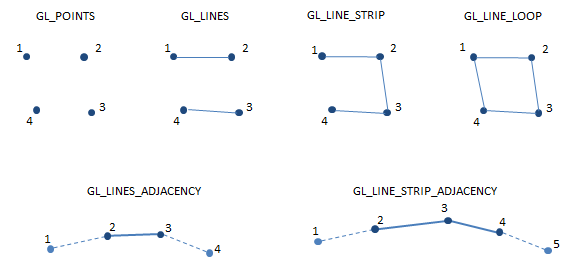
\includegraphics[scale=0.7]{02theorie/openglPrimitives.png}
	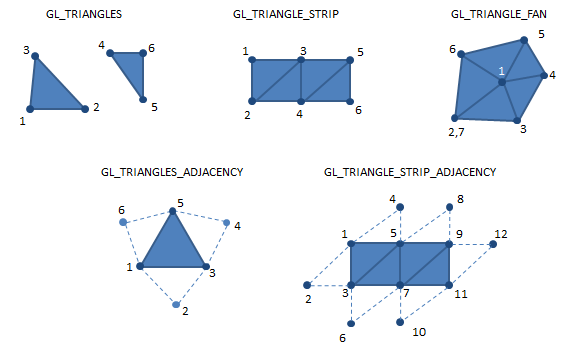
\includegraphics[scale=0.7]{02theorie/openglPrimitives2.png}
	
	
	Quelle: http://www.lighthouse3d.com/tutorials/glsl-tutorial/primitive-assembly/
	\caption{OpenGL Primitives}\label{OpenGLPrimitives}
\end{figure}


\begin{figure}
	\centering
	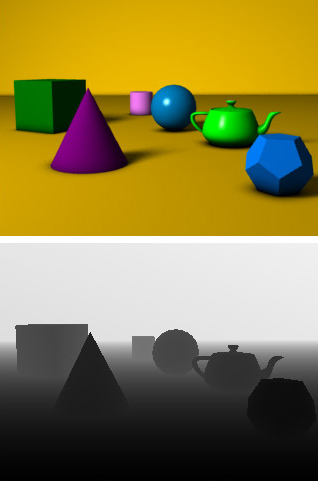
\includegraphics[scale=0.5]{02theorie/DepthBuffer.jpg}
	
	
	Oben: Color, Unten: Depth
	
	Quelle: https://de.wikipedia.org/wiki/Datei:Z-buffer\textunderscore no\textunderscore text.jpg
	\caption{Color- und Depth-Buffer}\label{DepthBuffer}
\end{figure}


\begin{figure}
	\centering
	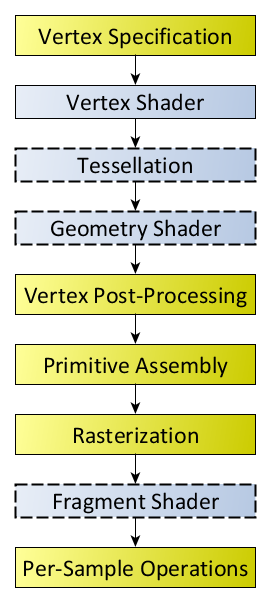
\includegraphics[scale=0.4]{02theorie/RenderingPipeline.png}
	
	
	Quelle: https://www.khronos.org/opengl/wiki/Rendering\textunderscore Pipeline\textunderscore Overview
	\caption{OpenGL Pipeline}\label{RenderingPipeling}
\end{figure}
\subsection{Physically Based Rendering}

In einer 3D-Szene eines Videospiels will man natürlich komplexere Objekte als Primitives darstellen. Diese Objekte bestehen aus vielen Primitives, wobei als Primitive Dreiecke genommen werden. Die Art der Zusammensetzung ist unterschiedlich, manchmal kann es von Vorteil sein aneinander hängende Dreiecke zu verwenden, aber meistens werden einfach einzelne Dreiecke gerendert. Einige Programme verwenden auch andere Polygone, aber diese bestehen auch nur aus Dreiecken, daher macht das keinen Unterschied. Ein Objekt, gebildet aus Dreiecken, nennt man \textit{Mesh}. Als Beispiel ist das Mesh eines Delfins in \cref{Dolphin} dargestellt. Die Farbe eines Objektes wird aus einem 2D Bild gelesen, genannt \textit{Textur}. Dafür besitzt jeder Vertex zusätzlich zu seiner Position eine 2D-Position auf der Textur, so kann ermittelt werden welche Pixel der Textur verwendet werden sollen. Mit Mesh und Textur ist es möglich ein Objekt in einer 3D-Szene anzuzeigen, aber es würde in einem Videospiel nicht überzeugen, da kommt \ac{PBR} ins Spiel. \ac{PBR} ist eine Möglichkeit eine realistischere 3D-Szene zu erzeugen in dem physikalische Phänomene wie Licht berücksichtigt werden. Wie ein Objekt auf Licht reagiert, hängt von verschiedenen Größen ab, wie die eigentliche Farbe des Objekts, die Oberflächenstruktur, aber auch die Farbe und Richtung des einfallenden Lichts. Alle Eigenschaften eines Objekts die sich auf die Farbe auswirken werden in einem \textit{Material} zusammengefasst. Ein zurenderndes  Objekt besitzt beides: ein Mesh und ein Material, was zusammengefasst \textit{Model} genannt wird.

Es gibt zwei Arten von Lichtquellen in der FM3D-Engine: \textit{Directional Light} und \textit{Point Lights}. Eins Directional Light besitzt, wie der Name sagt, eine Richtung aber keine Position. Es kann verwendet werden um zum Beispiel die Sonne darzustellen. Diese ist soweit von der Erde entfernt, dass die Position irrelevant ist, die Richtung dagegen ist wichtig und von der Tageszeit abhängig. Point Lights sind das genaue Gegenteil Sie besitzen keine Lichtrichtung sondern scheinen in alle Richtungen gleich, dafür besitzten sie aber eine genau festgelegte Position, welche wichtig ist, da die Lichtstärke mit zunehmendem Abstand kleiner wird. Point Lights können verwendet werden um die meisten Lichtquellen darzustellen wie Laternen oder Fackeln. Man kann aber nicht nur zwischen Lichtquellen unterscheiden sondern auch zwischen verschiedenen Arten des ausgesendeten Lichts. Die FM3D-Engine verwendet ein Lichtmodell genannt "Ambient/Diffuse/Specular". \textit{Ambient light} ist das Licht welches man jeden Tag sieht, auch wenn gerade keine Sonne scheint oder man sich nicht in direkter Nähe einer Lichtquelle befindet. Es entsteht dadurch, dass Licht von allen Objekten wieder teilweise reflektiert wird und so eine schwache und gleichmäßige Beleuchtung entsteht. Ohne diese wäre es hinter einem Haus, welches die Sonne verdeckt, komplett finster. Die zweite Lichtart ist \textit{Diffuse light}, welches abhängig von dem Auftrittswinkel des Lichtstrahls ist. Die dem Licht zugewandte Seite eines Würfels heller ist als die nur teilweise zugewandte Seite und die abgewandte Seite erfährt gar kein Diffuse light. \textit{Specular light} modelliert die Lichtstrahlen, welche von einem Objekt reflektiert und in die Linse der Kamera bzw. in die Augen des Betrachters gelangen. Dies wird als blendendes, helles Licht wahrgenommen und ist oft auf metallischen Obeflächen zu erkennen. Diese drei Lichtarten sind in \cref{Img:Lights} dargestellt.

Alle Lichtberechnungen müssen für jeden Pixel ausgeführt werden und laufen daher im Fragment shader ab.
Um die Farbe eines gerenderten Pixels zu bestimmen benötigen wir einige Informationen: Die Position des Pixels, die Farbe des Pixels, den Normalenvektor des Pixels und Specular factor des Pixels. Diese 4 Informationen reichen für alle Lichtberechnungen aus. Die Phase in der sie erstellt bzw. berechnet werden ist unterschiedlich. Ein Teil wird außerhalb des Programms in externen Programmen erstellt und als Vertex im Mesh oder als Information im Material. Dabei kann man unterscheiden zwischen: Information die sich zwischen verschiedenen Objekten unterscheidet aber nicht innerhalb des Objekts, Information die für jeden Vertex anders ist aber für jeden Pixel nur linear interpoliert werden muss und Information die für jeden Pixel anders ist. Ersteres ist das einfachste und kann einfach im Material gespeichert werden, da jedes Objekt ein eigenes Material haben kann und es anders als ein Mesh nicht viel Speicher benötigt. Die Vertexinformationen werden im \ac{VBO} des Mesh gespeichert und automatisch linear interpoliert wenn sie an den Fragment shader weiter gegeben werden. Pixelinformationen müssen einzeln in einer Textur gespeichert werden, diese ist dann im Material enthalten, wobei sie nur referenziert wird, damit verschiedene Materials die gleichen Texturen verwenden können. In den Vertexinformationen müssen hierfür zusätzlich Texturkoordinaten gespeichert werden. Daraus ergeben sich die folgenden Werte:

\begin{table}
	\caption{Vertex Aufbau}
	\label{table:VertexAufbau}
	\centering
	\begin{tabular}{lll}\toprule[1.5pt]
		Datentyp & Name & Beschreibung \\\midrule
		3D-Vektor & Position & Position des Vertex \\
		2D-Vektor & Textur Koordinate & Position des Vertex auf der Textur \\
		3D-Vektor & Normal & Normalenvektor zum Dreieck \\
		32-Bit Farbe & Color & Farbe des Vertex (optional, Standard ist weiß) \\
		3D-Vektor & Tangent & Tangentenvektor des Dreiecks. Benötigt wenn \\
		 & & Normal maps verwendet werden. Siehe \cref{section:Normalmapping}\\\bottomrule[1.5pt]
	\end{tabular}
\end{table}
\begin{table}
	\caption{Material Aufbau}
	\centering
	\begin{tabular}{lll}\toprule[1.5pt]
	Datentyp & Name & Beschreibung \\\midrule
	32-Bit Farbe & Color & Farbe des gesamten Objekts \\
	Textur & Color Texture & Gibt die Farbe jedes Pixels des Objektes an \\
	Textur & Normal map & Gibt den Normalenvektor jedes Pixels an. \\
	 & & Genaueres in \cref{section:Normalmapping} \\
	Float & Specular factor & Faktor für das resultierende Specular light \\
	Textur & Specular map & Specular factor für jeden Pixel. Der Faktor \\
	 & & des ganzen Objekts wird weiterhin verwendet \\
	 Boolean & UseWireframe & Gibt an ob ganze Dreiecke gerendert werden sollen\\
	  & & oder nur die Kanten. (Nützlich für Debugging)\\\bottomrule[1.5pt]
\end{tabular}
\end{table}


\begin{figure}
	\begin{center}
		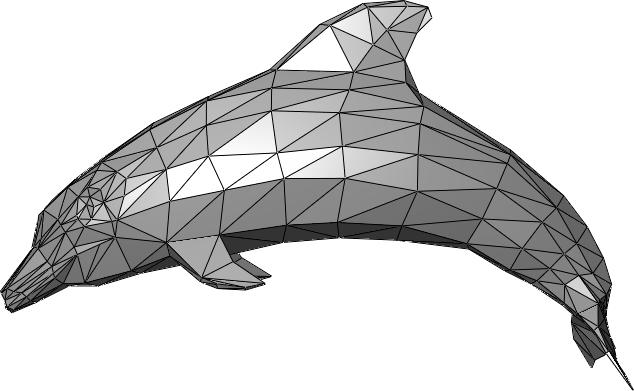
\includegraphics[width=0.5\textwidth]{06anhang/bilder/delphin.jpg}
		\caption{Mesh eines Delfins}
		\label{Dolphin}
	\end{center}
\end{figure}
\begin{figure}
	\centering
	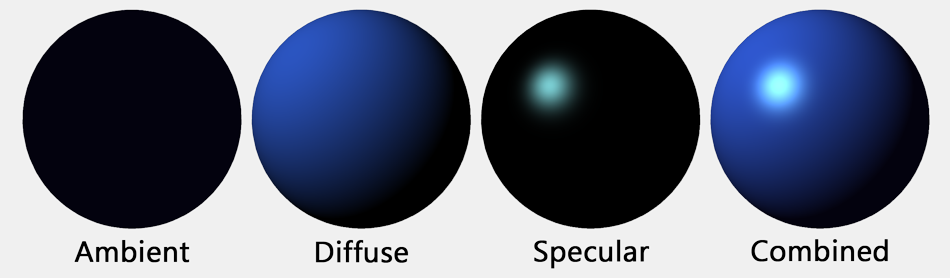
\includegraphics[scale=0.4]{02theorie/amb_diff_spec.png}
		
	Quelle: https://clara.io/img/pub/amb\textunderscore diff\textunderscore spec.png
	\caption{Lights}\label{Img:Lights}
\end{figure}
\subsection{Normalmapping}
\label{section:Normalmapping}

Um die visuelle Qualität eines Models zu erhöhen, so muss man das Modell genauer modellieren und somit resultieren mehr Dreiecke. 
Damit erhöht sich aber auch der Rechenaufwand für dieses Model und ab einer bestimmten Grenze ist die gewonnene Qualität nur sehr gering, der Rechenaufwand aber um so größer. Um ein Model trotzdem noch hochauflösender darzustellen wird ein Vorgang namens \textit{Normalmapping} verwendet. 
Dieser baut auf Lichtberechnungen auf, denn ohne Licht gibt es keine zu erkennende verbesserte Qualität. Normalerweise hat jeder Vertex einen Normalenvektor und für einen Pixel wird er zwischen den 3 Vertices interpoliert. Mit Normalmapping weißt man jedem Pixel einen eigenen Normalenvektor zu, so ist es möglich die Oberfläche so aussehen zu lassen, als würde sie rau mit kleinen Unebenheiten sein, ohne den Rechenaufwand von dem Rendern vieler Dreiecke eines Meshes zu belasten.
Den Unterschied Sieht man in \cref{img:Normalmapping}. Die Normalenvektoren werden in einer Textur gespeichert, sodass sie mit den normalen Texturen-Koordinaten verwendet werden können. Diese Textur wird im Material abgespeichert.

In einer Textur können drei Werte abgespeichert werden, Rot, Grün und Blau, jeweils mit einem Wert von 0 bis 1. Ein Normalenvektor hat aber drei Komponenten mit jeweils Werten von -1 bis 1, daher muss dieser erst berechnet werden:

$ \overrightarrow{N} = 
\begin{pmatrix}
x \\ y \\ z
\end{pmatrix}
 = 2 \cdot \overrightarrow{C} - 1 = 
 \begin{pmatrix}
 2 \cdot r - 1 \\ 2 \cdot g - 1 \\ 2 \cdot b - 1
 \end{pmatrix}$
 
Der Normalenvektor $\begin{pmatrix}
	0 \\ 0 \\ 1
\end{pmatrix}$ zeigt direkt weg von dem Model, daher sind Normalmaps auch immer sehr bläulich, denn der meiste Anteil des Normalenvektors liegt in der Z-Komponente. Eine Beispiel Normalmap ist in \cref{img:Normalmap} zu sehen. Man kann diesen Vektor aber nicht direkt verwenden, da er im \textit{Tangent space} definiert ist. Dies bedeutet dass er relativ zu dem zugehörigen Dreieck steht.
Man benötigt zudem einen Normalenvektor im \textit{Object space}, also relativ zu dem Model. 
Zur Umwandlung wird eine 3x3 Matrix benötigt, die aus drei verschiedenen Vektoren des Tangent-Space gebildet wird. 
Es können hierbei drei beliebige nicht linear abhängige Vektoren verwendet werden. Man bemerkt schnell, dass wenn alle drei orthogonal zueinander verlaufen, es simpler und effizienter ist die Matrix zu erstellen. 
Der erste Vektor wird bereits angegeben. Dieser beschreibt den Standardnormalenvektor jedes Vertex. Hinzu kommt noch ein Tangentenvektor jedes Vertex. Dieser befindet sich ebenfalls im \ac{VBO} des Meshes, wie in \cref{table:VertexAufbau} abgebildet ist. Der dritte Vektor ist der Bitangentenvektor
und kann mittels Kreuzprodukt aus diesen beiden berechnet werden. Es ist nötig alle drei Vektoren zu normalisieren, bevor die Matrix erstellt wird.

Gegeben ist der Normalenvektor $\overrightarrow{N}$ und der Tangentenvektor $\overrightarrow{T}$

Die normalisierten Vektoren: $\overrightarrow{N_{0}} = \dfrac{\overrightarrow{N}}{|\overrightarrow{N}|}$\qquad	$\overrightarrow{T_{0}} = \dfrac{\overrightarrow{T}}{|\overrightarrow{T}|}$

Der Bitangentenvektor: $\overrightarrow{B} = \overrightarrow{N_{0}} \times \overrightarrow{T_{0}}$\qquad	$\overrightarrow{B_{0}} = \dfrac{\overrightarrow{B}}{|\overrightarrow{B}|}$

Die Matrix sieht dann so aus: $M =  \begin{pmatrix}
T_{0x} & B_{0x} & N_{0x} \\
T_{0y} & B_{0y} & N_{0y} \\
T_{0z} & B_{0z} & N_{0z} \\
\end{pmatrix}$

Diese Matrix wird für erhöhte Leistung im Vertex shader erstellt und dann dem Fragment shader übergeben. In diesem muss dann nur der Normalenvektor aus der Normalmap geladen werden, dafür werden die gleichen Texturekoordinaten verwendet wie bei der Color texture, und mit dieser Matrix multipliziert werden.

\begin{figure}
	\begin{center}
		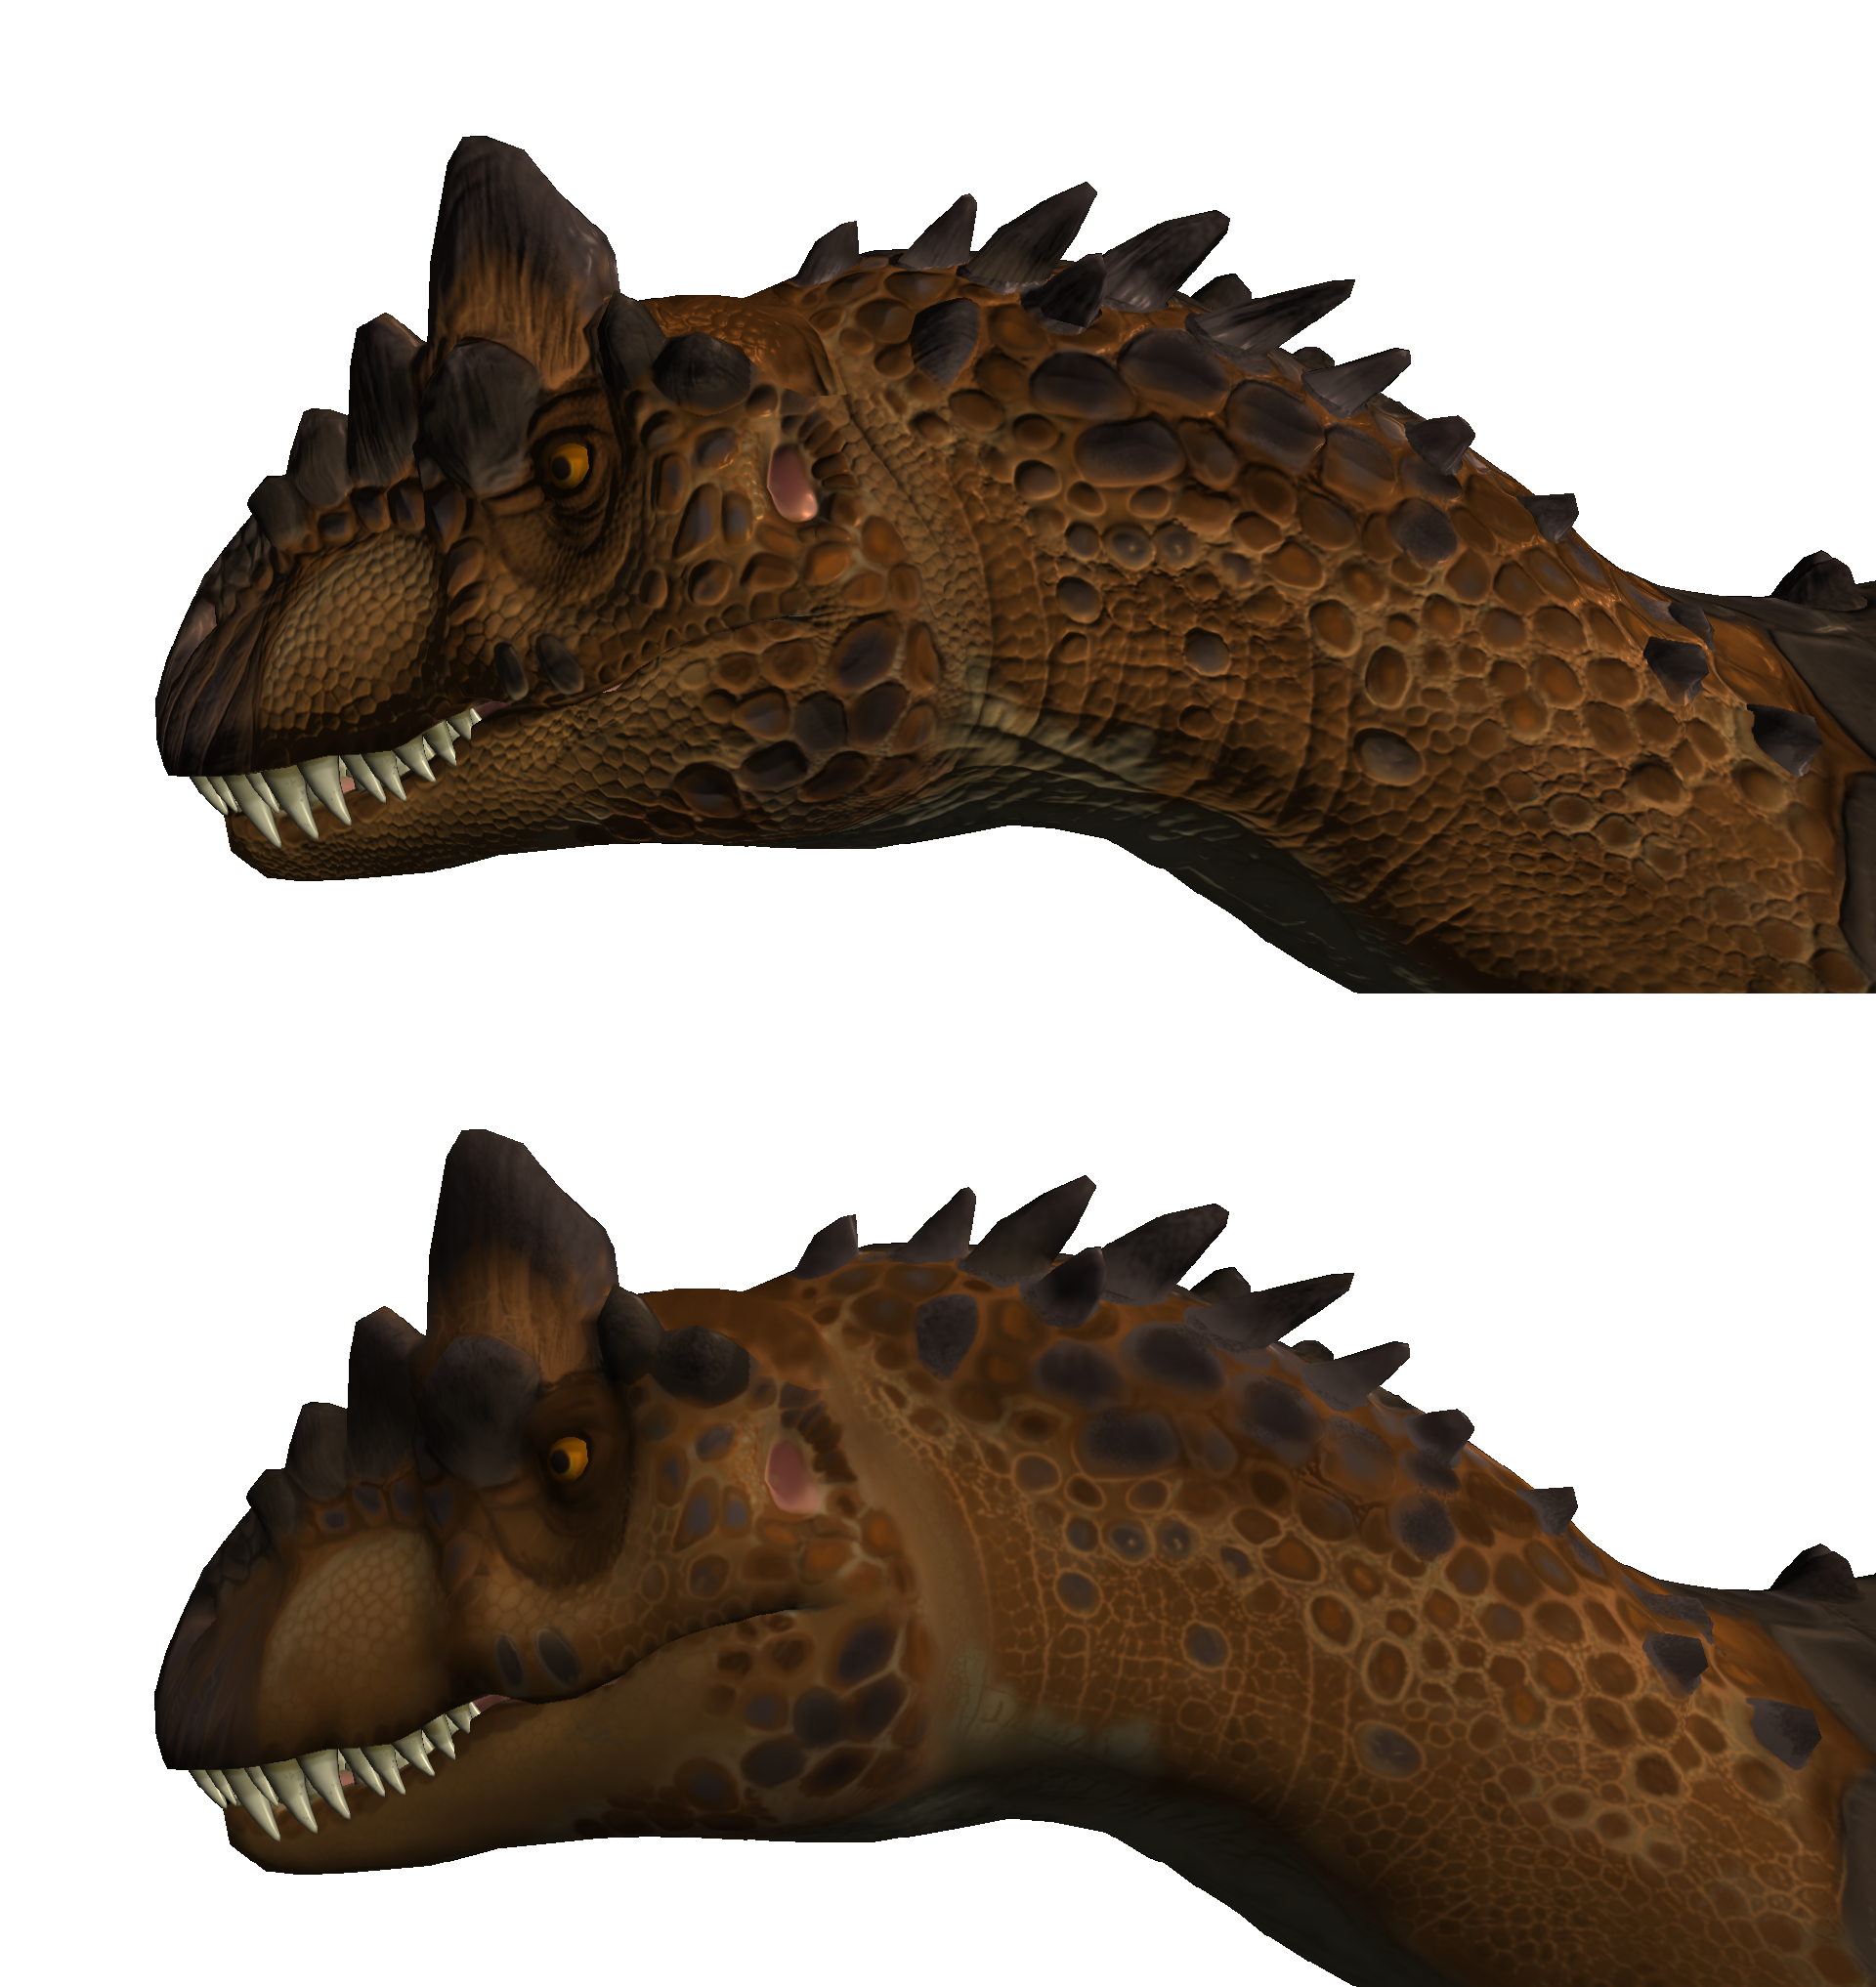
\includegraphics[width=0.5\textwidth]{02theorie/Normalmapping.png}
		
		Oben: mit Normalmapping, Unten: ohne Normalmapping
		
		Model: Allosaurus aus dem Spiel "`Ark: Survival Evolved"
		
		\caption{Normalmapping Beispiel}
		\label{img:Normalmapping}
	\end{center}
\end{figure}
\begin{figure}
	\begin{center}
		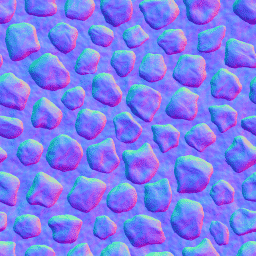
\includegraphics[width=0.4\textwidth]{02theorie/normalmap.png}
		
		Eine Beispiel Normalmap
		
		Quelle: http://www.bencloward.com/images/tutorial\textunderscore normals07.gif
		
		\caption{Normalmap Beispiel}
		\label{img:Normalmap}
	\end{center}
\end{figure}
\subsection{Animation}

Für einer lebendige Szene in einem Spiel reicht es nicht aus nur statische Models zu verschieben und zu drehen. Wenn man zum Beispiel ein Pferdmodel im Spiel einbindet und es nur nach vorne bewegt, wenn es laufen soll, so wirkt das Pferd nicht lebendig und es sähe so aus als würde man eine Statue verschieben. Man muss in diesem Falle also ein Modell animieren.
Die FM3D-Engine verwendet eine Animationsart namens \textit{Skeletal-Animation}. Hierbei bekommt jedes animierte Mesh ein Skelett zugewiesen, wobei sich mehrere verschiedene Meshes das gleiche Skelett teilen können. Zum Beispiel könnte es in einem Spiel ein Mesh für einen Ritter und eines für einen Bauern geben. Diese sehen unterschiedlich aus, aber beide könnten das gleiche Skelett haben und somit die gleichen Animationen.

Ein Skelett besteht aus mehreren Knochen, die jeweils weitere Knochen besitzen. Wenn sich ein Knochen bewegt, bewegt er alle an ihm hängende Knochen und die wiederum alle an ihnen hängenden. 
Dies hat den Vorteilm, dass wenn sich der Knochen des linken Armes bewegt, sich auch gleichzeitig alle Fingerknochen bewegen würden. Jeder Knochen besitzt unabhängig von den anderen eine Ausgangsposition und eine ID.
Die Id wird verwendet um herauszufinden, welcher Knochen sich auf welchen Vertex auswirkt und welche Knochen gar nicht verwendet werden. Jeder Vertex kann von bis zu 4 Knochen transformiert werden. Dazu besitzt jeder Vertex 4 Knochen-IDs und 4 floats die angeben wie stark sich ein Knochen auf den Vertex auswirkt, wie in \cref{table:VertexAufbau} zu sehen ist. Diese Daten werden in einem externen Programm beim Erstellen des Meshes festgelegt. Dieser Vorgang wird \textit{Weight painting} genannt, da die Zuweisung durch eine Art Malen in den Modellierungsprogrammen geschieht. Ein Beispiel aus dem Programm Blender ist in \cref{Img:Skeleton} zu sehen.

Eine Animation besitzt zu verschiedenen Zeitpunkten eine Position, Rotation und Skalierung für einen Knochen genannt \textit{Keyframe}. Dabei ist es nicht nötig, dass alle Knochen die gleiche Anzahl an Keyframes haben oder einen Keyframe an der gleichen Zeitposition. Es ist auch möglich, dass Keyframes nicht Position, Rotation und Skalierung auf einmal beinhalten sondern nur eins oder zwei davon. Um den Zustand aller Knochen zu einem bestimmten Zeitpunkt herauszufinden fängt man am obersten Knochen der Hierarchie an und arbeitet sich dann schrittweise nach unten, da die unteren Knochen von den oberen abhängig sind. 
Falls der Zustand zu diesem Zeitpunkt nicht zufällig durch die Keyframes genau definiert ist, muss zwischen den zwei am nächsten liegenden Keyframes interpoliert werden.

Für die Position und Skalierung kann zwischen den Keyframes linear interpoliert werden:

$t_{0} \leq t \leq t_{1}$ \qquad $t_{0} < t_{1}$ \qquad Keyframes: $\overrightarrow{P_{0}}, \overrightarrow{P_{1}}$

$f = \dfrac{t - t_{0}}{t_{1} - t_{0}}$

$\overrightarrow{P} = ((\overrightarrow{P_{0}} \cdot (1 - f)) + (\overrightarrow{P_{1}} \cdot f)$

Für die Rotation muss \ac{SLERP}\cite{WikiSlerp} angewendet werden, dadurch bleibt die Kreisgeschwindigkeit über die Zeit konstant. Die Berechnung erfolgt für zwei Quaternionen, die eine Rotation repräsentieren.

$t_{0} \leq t \leq t_{1}$ \qquad $t_{0} < t_{1}$ \qquad Keyframes: $Q_{0}, Q_{1}$

$f = \dfrac{t - t_{0}}{t_{1} - t_{0}}$

$\phi = Q_{0} \cdot Q_{1}$

$\theta = \arccos(\phi) \cdot f$

$Q_{2} = Q_{1} - Q_{0} \cdot \phi$

$Q = Q_{0} \cdot \cos(\theta) + Q_{2} \cdot \sin(\theta)$

\begin{figure}
	\centering
	\begin{minipage}{0.49\textwidth}
		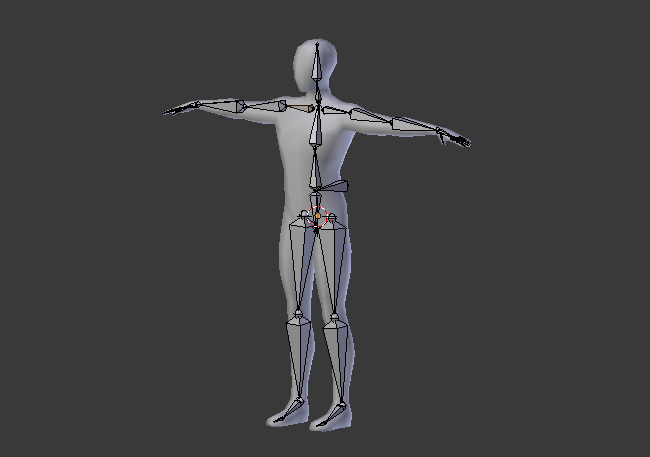
\includegraphics[width=\textwidth]{02theorie/skeleton.jpg}
	\end{minipage}
	\hfill
	\begin{minipage}{0.49\textwidth}
		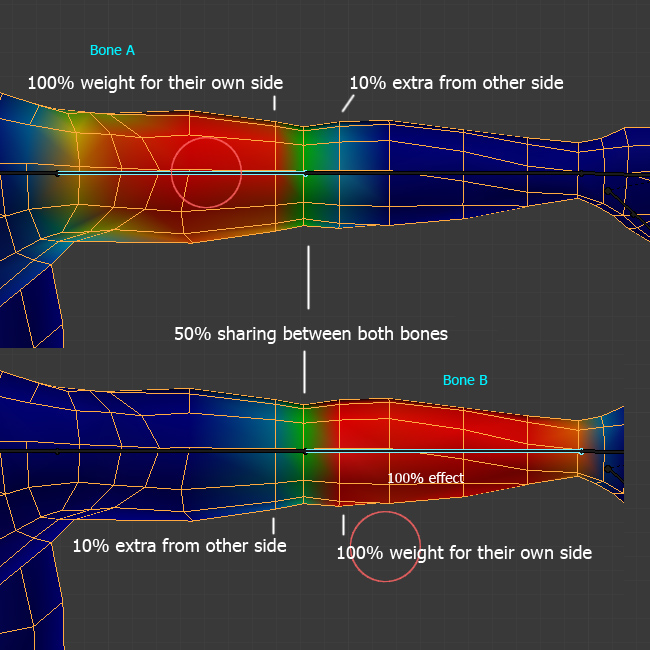
\includegraphics[width=\textwidth]{02theorie/weightpainting.jpg}
	\end{minipage}

	
	Links: Skelett in Blender, Rechts: Weight painting eines Arms in Blender 
	
	Quelle: https://cgi.tutsplus.com/tutorials/building-a-basic-low-poly-character-rig-in-blender--cg-16955
	\caption{Blender Skelett}\label{Img:Skeleton}
\end{figure}
\subsection{Projection Matrix}
\label{Sec:Projection}
Wenn man sich einen Computerbildschirm anschaut, so stellt man fest, dass er eine zweidimensionale Oberfläche besitzt. 
Da aber die zu rendernde Szene dreidimensional ist, muss man diese Szene, bestehend aus mehreren dreidimensional angeordneten Grafik-Primitiven, auf diese zweidimensionale Oberfläche projizieren. Dafür verwendet man eine sogenannte \textit{Transformation}.

Man kann sich das ganze so vorstellen, dass eine simulierte ideale Version einer Loch-Kamera mit einem unendlich kleinen Loch verwendet wird. Dies bedeutet, dass alle Objekte scharf dargestellt werden. Da eine Lochkamera aber das Bild verkehrt herum abbildet, wird der Einfachheit wegen die Bildebene vor dem Projektionszentrum abgebildet. Somit steht das Bild nun nicht mehr auf dem Kopf und muss nicht mehr invertiert werden. \cref{lochkamera}

Wenn wir uns nun einen Punkt $P(p_{x}, p_{y}, p_{z})$ in der Szene anschauen, so geht durch diesen vom Projektionszentrum aus bis zum projizierten Punkt auf dem Bildschirm $P'(p'_{x}, p'_{y}, p'_{z})$ eine Gerade. Mit dem Strahlensatz lässt sich nun aus $\dfrac{p'_{x}}{\mathnormal{f}} = \dfrac{p_{x}}{p_{z}} $ und $ \dfrac{p'_{y}}{\mathnormal{f}} = \dfrac{p_{y}}{p_{z}} $ die folgende Formel für Punkt $P$ bestimmen, die da lautet $P'=(\mathnormal{f}\dfrac{p_{x}}{p_{z}}, \mathnormal{f}\dfrac{p_{y}}{p_{z}}, \mathnormal{f})$.
Nun kann die Projektion in einer Matrix abgebildet werden.

Weil $$\mathbf{P'}= \begin{pmatrix} p'_x \\ p'_y \\ p'_z \end{pmatrix}= \begin{pmatrix} f
\frac{p_x}{p_z}\\ f \frac{p_y}{p_z}\\ f \end{pmatrix} \in \mathbb{R}^3 \longmapsto \underline{\mathbf{P'}}= \begin{pmatrix}f \, p_x \\f \, p_y \\ f \, p_z\\
p_z\end{pmatrix} \in \mathbb{H}^3 $$
gilt:	


\begin{align}\mathbf{\underline{P'}} & =
	\begin{pmatrix}f \, p_x \\f \, p_y \\ f \, p_z\\ p_z\end{pmatrix}  = \begin{bmatrix} f & 0 & 0 & 0 \\ 0 & f & 0 & 0 \\ 0 & 0 & f & 0 \\ 0 & 0 & 1 & 0 \end{bmatrix} \begin{pmatrix}p_x \\p_y
		\\ p_z\\ 1 \end{pmatrix} \end{align}

Da die Projektion von OpenGL aber auf die negative Z-Achse ausgerichtet ist, gilt dementsprechend
\begin{align}\mathbf{\underline{P'}} & =
	\begin{pmatrix}f \, p_x \\f \, p_y \\ f \, p_z\\ -p_z\end{pmatrix}  = \begin{bmatrix} f & 0 & 0 & 0 \\ 0 & f & 0 & 0 \\ 0 & 0 & f & 0 \\ 0 & 0 & -1 & 0 \end{bmatrix} \begin{pmatrix}p_x \\p_y
		\\ p_z\\ 1\end{pmatrix} \end{align}

In der 3D-Computergrafik und somit auch in OpenGL verwendet man sogenannte \textit{Near-/ Far-Clipping} Ebenen, welche parallel zur Projektion (dem Bildschirm) stehen. Diese beiden Ebenen sind für die Begrenzung der Sicht gedacht. Alle Modelle/Punkte, die sich vor der \textit{Near-Clipping} Ebene befinden, sind zu nah. Dies heißt, dass sie nicht angezeigt werden sollen. Alle Modelle/Punkte, die sich vor der \textit{Far-Clipping} Ebene befinden, sind zu weit entfernt und werden ebenfalls nicht angezeigt. (Siehe \cref{nfplane}) Mathematisch kann man dies nun so umsetzen: für die \textit{Near-Clipping} Ebene hieße das $p_z=-z_n \quad$, dies entspricht $p'_z=-1$ . Die \textit{Far-Clipping} Ebene wäre mit $p_z=-z_f \quad$ definiert, was auch als $p'_z=1$ geschrieben werden kann.

Zuerst nehmen wir uns die Parameter $a$ und $b$ in unsere bisherige Transformations-Matrix. 
\todo[inline]{TODO!}
%\url{http://www.mathematik.uni-marburg.de/~thormae/lectures/graphics1/graphics_6_1_ger_web.html#15}

\begin{figure}
	\centering
	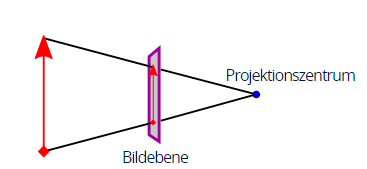
\includegraphics[scale=0.7]{02theorie/Lochkamera.png}
	Quelle: \url{http://www.mathematik.uni-marburg.de/~thormae/lectures/graphics1/graphics_6_1_ger_web.html#10}	
	11.01.2017
	\caption{Lochkamera in der Grafikprogrammierung}\label{lochkamera}
\end{figure}

\begin{figure}
	\centering
	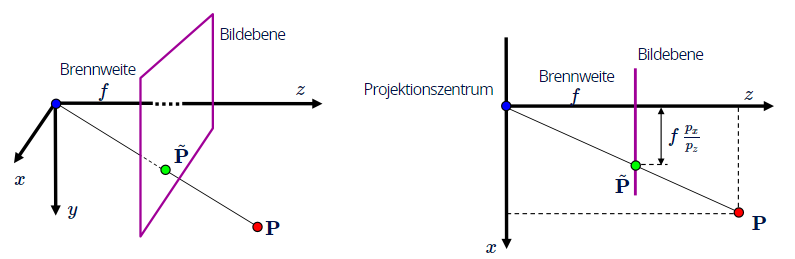
\includegraphics[scale=0.7]{02theorie/perspektivischeprojektion.png}
	Quelle: \url{http://www.mathematik.uni-marburg.de/~thormae/lectures/graphics1/graphics_6_1_ger_web.html#11}	
	11.01.2017
	\caption{Perspektivische Projektion}\label{perspproj}
\end{figure}

\begin{figure}
	\centering
	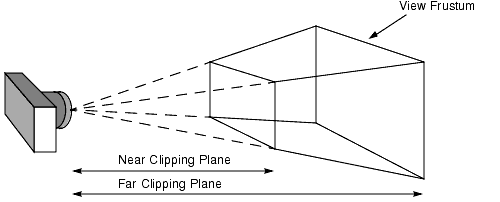
\includegraphics[scale=0.7]{02theorie/ViewModel11.png}
	Quelle: \url{http://download.java.net/media/java3d/javadoc/1.4.0/javax/media/j3d/doc-files/ViewModel11.gif}	
	14.01.2017
	\caption{Near-/Far-Clipping Plane}\label{nfplane}
\end{figure}


\section[Extensible Markup Language]{Extensible Markup Language\cite{xml}\cite{xmlcstutorials}\cite{msdn}}
\label{extensiblemarkuplanguage}

Im Designer wird häufig die \textit{Extensible Markup Language} (kurz \ac{XML}) verwendet.  Diese \textit{erweiterbare Auszeichnungssprache} wird im FM3D-Designer gebraucht, um in gespeicherten Dateien hierarchisch strukturiert Daten in Textdateien zu speichern.
Sowohl die Projektdateien, Entity-Dateien, Modeldateien uvm. werden in Form von \ac{XML} beschrieben. 
\ac{XML} beschreibt eine Baumstruktur von Daten die hierarchisch angeordnet sind. Ein \ac{XML}-Dokument besteht aus Elementen, Attributen, Verarbeitungsanweisungen und/oder Kommentaren. 
Ein Element kann mittels einem Paar aus Start-Tag (zB. \textit{<Tag>}) und End-Tag (zB. \textit{</Tag>}) oder einem leeren Tag (zB. \textit{<Tag/>}) erfolgen.
Diesen Elementen kann man nun beliebig viele Attribute zuordnen, welche wiederum Werte besitzen.
Die Werte der Attribute sind standardmäßig in Form des Datentyps \textit{String}. Dieser muss in C-Sharp zunächst in den benötigten Datentyp umgewandelt werden.
Als Beispiel wird nun das Dokument in \cref{xmlbsp} verwendet. 
In \cref{xmlbsp} erkennt man zunächst einen Verarbeitungshinweis, welcher die XML-Version und Zeichenkodierung spezifiziert. Das darauffolgende Element \textit{<Wald>} besitzt das Unterelement \textit{<Baum>}. Dieses Element besitzt das Attribut \textit{name} mit dem Wert \textit{Eiche}. 
Dieses Element \textit{<Baum>} enthält weitere drei Unterelemente als leere Tags. Sie besitzen keine weiteren Unterelemente. Das Element \textit{<Stamm>} besitzt das Attribut \textit{LängeInMeter} mit dem Wert \textit{"`3"'}. Möchte man diesen Wert als Integer in C-Sharp verwenden, so muss man diesen String erst in einen solchen Typ konvertieren. Des weiteren besitzt das Element \textit{<Baum>} noch zwei Unterelemente mit dem Namen \textit{<Blatt>}. Beide dieser besitzen das Attribut \textit{Farbe}. Auch hier liegt der Wert als String vor.
In \cref{fm3dprojekt} wird ein kommentiertes FM3D-Projekt dargestellt. Die Kommentare werden nicht in der Datei gespeichert und sind nur für die Veranschaulichung abgebildet.
\begin{figure}
	\begin{center}
		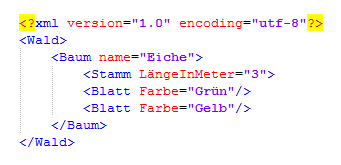
\includegraphics[width=0.6\textwidth]{03unserprogramm/Designer/xmlbsp.png}
		\caption{XML-Beispiel}\label{xmlbsp}
	\end{center}
\end{figure}
\begin{figure}
	\begin{center}
		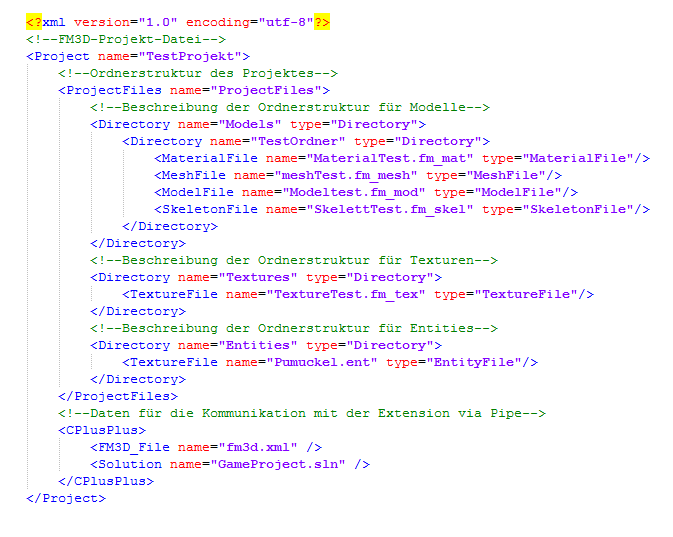
\includegraphics[width=\textwidth]{03unserprogramm/Designer/FM3DProjektdatei.PNG}.
		\caption{FM3D-Projektdatei, welche vom Designer erstellt und gespeichert wird}\label{fm3dprojekt}
	\end{center}
\end{figure}
\chapter{Unser Programm}
\label{c:unserprogramm}
\section{Engine - Allgemeiner Aufbau}

Die Engine ist eine Visual C++ Laufzeitbibliothek (Dynamic-Link-Library; DLL). Diese DLL enthält den gesamten Code, welcher zum Erstellen eines Spieles erforderlich ist. Jason Gregory beschreibt in seinem Buch den Aufbau einer Game-Engine als eine Struktur aus Systemen und Schichten. 
Hierbei können mehrere Schichten übereinander liegen. Ideal verwenden die höher gelegenen Schichten bereitgestellte Funktionalitäten der unteren Schichten, was aber nie umgekehrt geschehen soll. Dies ermöglicht die Abschirmung von hardwareabhängigen und spielnahen Klassen. Ein System übernimmt eine bestimmte Aufgabe und kann sich über mehrere Schichten ausbreiten. \cite{gea}
Die FM3D-Klasse hat diese Idee in bestimmten Teilen übernommen. Im Code ist die System-Struktur als Ordner-Struktur wiederzufinden. Diese Systeme sind teilweise auch durch einen \textit{Namespace} oder Präfix vor jedem Namen zu erkennen. Das Schichtenmodell ist in der Engine als mehrere Untersysteme (auch Subsystems genannt) erkennbar. Diese Untersysteme sind genauso zu erkennen und verhalten sich wie normale Systeme. Der einzige Unterschied ist, dass sie sich bereits in einem System befinden.
\section{Engine - Systeme}
\subsection{Math System}

Das Math-System ist für sämtliche mathematischen Berechnungen zuständig. Dazu gehören sehr einfache Rechnungen wie Umwandlung von Grad in Bogenmaß, aber auch komplexere Rechnungen wie zum Beispiel Matrix-Rechnungen. 
Das System besteht aus Klassen, aber auch einigen C-Style Funktionen, welche kleine Berechnungen ausführen, wie das Umwandeln von Grad in Bogenmaß. Alle Klassen sind Templateklassen, damit sie so flexibel wie möglich sind und für verschiedene Zahl-Datentypen verwendet werden können. Auf Vererbung wurde komplett verzichtet, da es wichtig ist alle Berechnungen so schnell wie möglich auszuführen. Statt Vererbung wird daher Template-Spezialisierung verwendet. Dies hat zwar den Nachteil, dass einiger Code mehrfach geschrieben, bzw. kopiert werden musste, aber dafür werden keine virtuellen Methoden verwendet und somit ist die Größe eines Objektes genau definiert. Dies ist wichtig, da einige Objekt in großer Anzahl in einem Buffer verwendet werden, in welchem alle Objekte im Speicher direkt aneinander liegen. Alle Klassen und Funktionen befinden sich im Namespace FM3D::Math, alle Typdefinitionen nur im Namespace FM3D für leichteren Zugriff.

Die zwei Grund Klassen sind Vector und Matrix. Sie besitzen jeweils einen Templateparameter für den Zahl-Datentyp der intern verwendet wird, dazu besitzen sie Ganzzahltemplateparameter, welche die Größe bzw. die Dimension angeben. Vector kann für alle Dimensionen sämtliche mathematischen Grundoperationen und zusätzlich einige Operationen, welche mathematisch nicht möglich sind, im Programm nützlich sind (Kursiv markiert), durchführen:

	\begin{longtable}[l]{ll}
		$\bullet$ Vektor-Addition		& $\overrightarrow{a} + \overrightarrow{b} = \begin{pmatrix} a_{0} + b_{0} \\ a_{1} + b_{1}\\ \vdots  \end{pmatrix} = \overrightarrow{c}$ \\
		$\bullet$ Vektor-Subtraktion	& $\overrightarrow{a} - \overrightarrow{b} = \begin{pmatrix} a_{0} - b_{0} \\ a_{1} - b_{1}\\ \vdots  \end{pmatrix} = \overrightarrow{c}$ \\
		$\bullet$ \textit{Vektor-Multiplikation} & $\overrightarrow{a} \cdot \overrightarrow{b} = \begin{pmatrix} a_{0} \cdot b_{0} \\ a_{1} \cdot b_{1}\\ \vdots  \end{pmatrix} = \overrightarrow{c}$ \\
		$\bullet$ \textit{Vektor-Division} & $\dfrac{\overrightarrow{a}}{\overrightarrow{b}} = \begin{pmatrix} a_{0} / b_{0} \\ a_{1} / b_{1}\\ \vdots  \end{pmatrix} = \overrightarrow{c}$ \\
		$\bullet$ \textit{Skalar-Addition}		& $\overrightarrow{a} + b = \begin{pmatrix} a_{0} + b \\ a_{1} + b\\ \vdots  \end{pmatrix} = \overrightarrow{c}$ \\
		$\bullet$ \textit{Skalar-Subtraktion}	& $\overrightarrow{a} - b = \begin{pmatrix} a_{0} - b \\ a_{1} - b\\ \vdots  \end{pmatrix} = \overrightarrow{c}$ \\
		$\bullet$ Skalar-Multiplikation	& $\overrightarrow{a} \cdot b = \begin{pmatrix} a_{0} \cdot b \\ a_{1} \cdot b\\ \vdots  \end{pmatrix} = \overrightarrow{c}$ \\
		$\bullet$ Skalar-Division		& $\dfrac{\overrightarrow{a}}{b} = \begin{pmatrix} a_{0} / b \\ a_{1} / b\\ \vdots  \end{pmatrix} = \overrightarrow{c}$ \\
		$\bullet$ Vektor-Produkt		& $\overrightarrow{a} \cdot \overrightarrow{b} = a_{0}b_{0} + a_{1}b_{1} + \dots = c$\\
		$\bullet$ Länge		& $|\overrightarrow{a}| = \sqrt{a_{0}^{2}+a_{1}^{2}+\dots} = c$\\
		$\bullet$ Normalisieren			& $\dfrac{\overrightarrow{a}}{|\overrightarrow{a}|} = \overrightarrow{a}$\\
		$\bullet$ Quadrierte Länge		& $|\overrightarrow{a}|^{2} = a_{0}^{2}+a_{1}^{2}+\dots = c$\\
	\end{longtable}

Diese Operationen sind als Methoden implementiert bei denen das Objekt, welches die Methode ausführt, am Ende dem neuen Vektor entspricht, also $\overrightarrow{a} = \overrightarrow{c}$. Zurückgegeben wird eine Referenz auf das Objekt, damit die Methoden aneinander gekettet werden können. Außerdem sind die Operationen als statische Methoden implementiert, welche den Vektor $\overrightarrow{a}$ und  $\overrightarrow{b}$ bzw. $b$ als Parameter annimmt und ein neues Objekt zurückgibt, ohne die Argumente zu verändern. Zusätzlich ist für jede Methode der entsprechende Operator als inline Methode bzw. inline friend Funktion implementiert. Dieser ruft einfach nur die Methode auf, sieht aber besser aus im Code.

Für Vektoren mit der Dimension zwei, drei und vier gibt es jeweils eine Spezialisierung der Template-Klasse. Das hat den Vorteil, dass die Member-Variablen richtige Namen haben und somit keine For-Schleifen verwendet werden müssen und die Klasse besitzt Methoden, welche nur für diese Dimension Anwendung finden. Dies sind zum Beispiel statische Methoden für die Koordinatenachsen oder das Kreuzprodukt für einen 3D-Vektor.

Die Matrix-Klasse verhält sich ähnlich wie die Vector-Klasse. Alle Elemente werden in einem Array gespeichert. Sie werden Reihe für Reihe gespeichert, was die folgenden Indices ergibt: \newline
$\begin{pmatrix}
	0 & 1 & 2 & 3 \\
	4 & 5 & 6 & 7 \\
	8 & 9 & 10 & 11 \\
	12 & 13 & 14 & 15
\end{pmatrix}$

 Die Klasse kann die folgenden Operationen ausführen:
\begin{itemize}
	\item Matrix-Multiplikation
	\item Matrix-Addition
	\item Skalar-Multiplikation
	\item Vektor-Multiplikation
\end{itemize}
Sie sind wie bei der Vector-Klasse als Methoden und Operatoren implementiert.

Es gibt zwei verschiedene Matrix-Spezialisierungen: Eine 2x2 Matrix und 4x4 Matrix.
Diese Klassen besitzen zusätzlich statische Methoden um spezielle Matrizen zu erstellen. Die 2x2 Matrix kann eine Rotationsmatrix für 2D-Vektoren erstellen, die 4x4 Matrix verschiedene Transformationsmatrizen für 3D-Vektoren:
	\begin{longtable}[l]{ll}
		$\bullet$ Projektionsmatrix & Siehe \cref{Sec:Projection}\\
		$\bullet$ Translationsmatrix & Verschiebung für $\overrightarrow{v} = \begin{pmatrix}
		x \\ y \\ z \\\end{pmatrix} \quad M = \begin{pmatrix}
		1 & 0 & 0 & x \\
		0 & 1 & 0 & y \\
		0 & 0 & 1 & z \\
		0 & 0 & 0 & 1
		\end{pmatrix}$\\
		$\bullet$ Rotationsmatrix & Berechnung nach \cite{WikiRotation}\\
		$\bullet$ Skalierungsmatrix & Faktoren: $x$, $y$, $z \quad M = \begin{pmatrix}
		x & 0 & 0 & 0 \\
		0 & y & 0 & 0 \\
		0 & 0 & z & 0 \\
		0 & 0 & 0 & 1
		\end{pmatrix}$\\
	\end{longtable}

 Bei der Multiplikation mit einem 3D-Vektor wird angenommen, dass die 4. Komponente des Vektors, welche nicht vorhanden ist, 1 beträgt. Dadurch ist es möglich Translationen abzubilden. Zusätzlich kann die 4x4 Matrix invertiert und transponiert werden.  

Damit nicht immer der volle Klassenname mit Templateargumenten ausgeschrieben werden muss, gibt es einige Typdefinitionen. Diese sind folgendermaßen aufgebaut:
\newline"`Vector"' + \textit{Dimension} + \textit{Abkürzung des Datentyps}
\newline"`Matrix"' + \textit{Anzahl Reihen} + \textit{Anzahl Spalten} + \textit{Abkürzung des Datentyps}
\newline Für quadratische: "`Matrix"' + \textit{Anzahl Reihen} + \textit{Abkürzung des Datentyps}
\newline"`Quaternion"' + \textit{Abkürzung des Datentyps}
\newline Zum Beispiel für einen dreidimensionalen Vektor mit dem Skalar-Datentyp \textit{float}: 
\newline\textit{Vector3f}
Zusätzlich gibt es noch Typdefinitionen für Farben. Diese sind nur eine andere Schreibweise eines Vektors bei der "Vector" mit "Color" ersetzt wird.

\subsection{File System}
Um Dateien verschiedener Formate in der FM3D-Engine verwenden zu können, wird die Klasse \textit{ExternFileManager} verwendet.
Die \textit{ExternFileManager} Klasse besitzt Methoden um Schriftarten, Bilder und Modelle zu laden. Der Methode \textit{ReadFontFile} um die Schriftarten zu laden übergibt man eine Referenz zu dem Namen der Datei. Zudem gibt man die Größe und die Skalierung der Schriftart an. Um die Textur auch in einem RenderSystem dar zu stellen, benötigt die Methode auch eine Referenz zu einem existierenden Objekt der \textit{RenderSystem}-Klasse. Die Methode benötigt zudem eine doppelte Referenz zu einem bereits erstelltes Objekt der Klasse \textit{Font}. 
Die Methode \textit{ReadTextureFile} gibt eine Referenz zu einem Objekt der Klasse Textur zurück. Als Übergabeparameter benötigt diese Methode zunächst das RenderSystem in dem die Textur gerendert werden soll. Außerdem benötigt diese Methode noch  die Enumerationen vom Typen \textit{FilterMode}, \textit{WrapMode} und \textit{MipMapMode}, welche in der Klasse \textit{Textur} stehen. Alle dieser Enumerationen besitzen bereits in dieser Methode einen Standardwert und müssen nicht explizit angegeben. Zur Erläuterung dieser Enumerationen siehe den \cref{Textureclass}. 
Die Methode \textit{ReadModelFile} benötigt als Übergabeparameter den Dateinamen, das RenderSystem in dem das Model geladen werden soll. Ein boolescher Übergabeparameter gibt an, ob \textit{Instancing} verwendet werden soll. Der darauffolgende  boolescher Wert gibt an, ob eine Animation in dem Model verwendet werden soll. Eine vierstellige Matrix \textit{Matrix4f} gibt die Skalierung des Models an.
Zur Initialisierung wird die Methode \textit{Initialize} verwendet.

\subsection{Graphic System}

\subsubsection{RenderSystem}
Um in diesem Fenster nun zu rendern benötigt man ein Objekt der Klasse RenderSystem. Das RenderSystem kontrolliert das Rendering der FM3D-Engine in der Anwendung. Diese Klasse besitzt eine Initialisierungsmethode, welcher man die Werte 

\subsubsection{Font-Klasse}
\label{Fontclass}
Objekte der Font-Klasse repräsentieren Schriftarten, welche man im Programm rendern kann.

\subsubsection{Texture-Klasse}
\label{Textureclass}
Die Klasse besitzt die Enumerationen \textit{FilterMode}, \textit{WrapMode} und \textit{MipMapMode}. In \textit{FilterMode} gibt verschiedene Filtermodi an, in denen die Textur gerendert wird.
Wenn verschiedene nebenstehende Pixel auf der Textur nicht auf den Bildschirm "'passen"` bzw. aufgrund der Transformation nicht parallel nebeneinander gerendert werden können, so muss zwischen den beiden Modi LINEAR und NEAREST auswählen. Der Modus NEAREST bildet eine Mischung der nebenstehenden Pixeln. 
Im Gegensatz du NEAREST bildet der Modus LINEAR bildet harte Kanten der gerendeten Textur.
Die Enumeration \textit{WrapMode} gibt an, wie die Textur auf das Modell gerendert werden soll und \textit{MipMap}.
Möchte man eine Textur für OpenGL erstellen, so verwendet man dafür die Klasse GL3Texture, welche von der Klasse Texture erbt. Diese Klasse beschreibt eine Textur, wie sie in OpenGL verwendet wird.

\subsubsection{Model-Klasse}
\label{Modelclass}
Die Klasse \textit{Model} besitzt alle Eigenschaften, die auch jedes andere Model besitzt. Darunter fällt ein Skelett, ein boolescher Wert, der angibt ob Instancing verwendet werden soll und die Anzahl der Teile. 
Der Begriff Instancing beschreibt das folgende:
Nehmen wir an, man rendert eine Szene mit einer Vielzahl an Modellen, welche eine Menge gleicher Vertices-Sätzen besitzen, aber eine andere Transformation besitzen.
Nehmen wir als Beispiel einen Baum:
Dieser Baum besitzt hunderte Blätter, welche alle gleich modelliert sind. Würde man ein einzelnes Blatt rendern, so würde dies sehr schnell verarbeitet werden. Aber die ganzen Render-Aufrufe verlangsamen das Programme um ein Vielfaches. 
Bei Instancing werden nun verschiedene Instanzen dieses Blattes gerendert. Dies spart eine Menge Zeit und lässt das Programm wesentlich schneller laufen.
Die Klasse \textit{AnimatedModel} erbt von der Klasse Model und beschreibt ein Model, welches animiert wird.

\subsubsection{Material-Klasse}
Um ein Modell zu rendern, so muss man ihm ein Material zuweisen. Jedes Model besteht aus verschiedenen Materialien welche von der Klasse Material beschrieben werden.
So kann man verschiedene Objekten die gleichen Materialien zuweisen. Möchte man zum Beispiel einen Tisch und einen Stuhl aus Holz rendern, so könnte man ein Material \textit{Holz} mit einer Textur, die \textit{Holz} abbildet. Dieses Material könnte man sowohl dem Tisch als auch dem Stuhl zuweisen.

\subsection{Entity System}
\label{entitysystem}
Bevor das Entity-System erläutert wird, muss erst geklärt werden, was ein Entity bzw. eine Entität überhaupt ist. Die Verwendung von Entities in der Engine werden im folgenden erläutert.
Peter Dr. Chen, welcher das Entity-Relationship-Model in den Jahren 1970 bis 1976 entwickelt wurde, definiert eine Entität als folgende:
\begin{quote}
	([...] Eine Entität ist ein "`Ding"', welche deutlich unterschieden werden kann. Als Beispiel für eine Entität kann zB. eine spezifische Person, Firma oder ein Event betrachtet werden. [...])
	(Aus \cite{entityrelationshipmodel}, Zitat aus dem Englischen übersetzt v. Max Schmitt)
\end{quote}
\todo[inline]{kann ich auf Homms blätter verweisen?}

Die FM3D-Engine verwendet ein \textit{Entity-Component-System} um Objekte eines Spieles zu verwalten. Im Gegensatz zu einem vererbungs-basierten Entity-System ist dieses sehr flexibel. 
Die Grundidee besteht darin, die \textit{Daten} und \textit{Logik} eines Entities aufzuteilen. Hierfür werden alle Daten eines Entities (alle Attribute eines Entities) in Komponenten geschrieben. %removed by max Variablen -> Attribute
Die Logik (Methoden, die das Entity ausführen soll) wird in einen Manager geschrieben. 
Ein Entity kann beliebig viele verschiedene Komponenten besitzen und sie können während der Laufzeit beliebig hinzugefügt oder entfernt werden. Jedoch kann ein Entity immer nur einen Komponente eines Typs enthalten. 
Der Manager führt dann bei jedem Update oder bei bestimmten Events eine Methode, das die vom Manager benötigten Komponenten enthält, für jedes Entity aus.

Alle Entities werden in einer \textit{Entity-Collection} gespeichert. Diese ist eine Sammlung von Entities, welche dafür zuständig ist neue Entities zu erstellen und alte zu löschen. Wenn ein Entity zerstört wird, so wird dieses nicht aus dem Speicher gelöscht. Es bleibt weiterhin in der Entity-Collection gespeichert. 
Wenn dann ein neues Entity erstellt wird, so muss nicht neuer Speicher angefragt werden und das bereits vorhandene aber "'gelöschte"` Entity kann nun wieder verwendet werden. Dies ermöglicht es sehr viel zeitsparender und effizienter eine hohe Anzahl von Entities zu erstellen und wieder zu löschen. 
Mit Komponenten verhält es sich genauso. In der \textit{Entity-Collection} werden alle zerstörten Komponenten gespeichert. Diese werden solange gespeichert, bis eine neue Komponente des gleichen Typs erstellt wird. Das gesamte Entity-System befindet sich im Namespace \textit{EntitySystem} um es vom restlichen Code abzutrennen.

Bevor wir auf die wichtigsten Klassen des Entity-Systems eingehen, müssen erst einige Hilfsklassen erläutert werden.
\todo[inline]{Erklärung von Events}

Dies wird im Code durch die folgende Klassenstruktur ermöglicht. Die Hauptklasse Entity besitzt einen Container mit Komponenten, welche nach ihrer ID sortiert sind. Um auf eine Komponente zuzugreifen, benötigt man nur die ID dieser in Form eines 32-Bit Integer. Auf diese kann man mit der Hilfsklasse \textit{ComponentIds} zugreifen. 
Diese Klasse enthält eine statische Variable, die jedes Mal bei einer neuen ID erhöht wird. Auf die ID kann dann mit der statischen Template-Methode Get() zugegriffen werden.
 
Um ein Entity zu erstellen benötigt man ein Objekt der Klasse \textit{EntityCollection}. Mit der Entity-Klasse selbst kann kein ein Objekt erstellt werden.  
Die \textit{EntityCollection} enthält eine \textit{Map} mit bereits gelöschten Komponenten um diese wiederverwenden zu können. 
Alle Komponenten müssen nach ihrer ID sortiert werden, da nur Komponenten, die mit dem neuen Typ übereinstimmen und daher die gleiche Speichergröße und Variablen haben, für den neuen Komponenten verwendet werden können.

\begin{figure}
	\begin{center}
		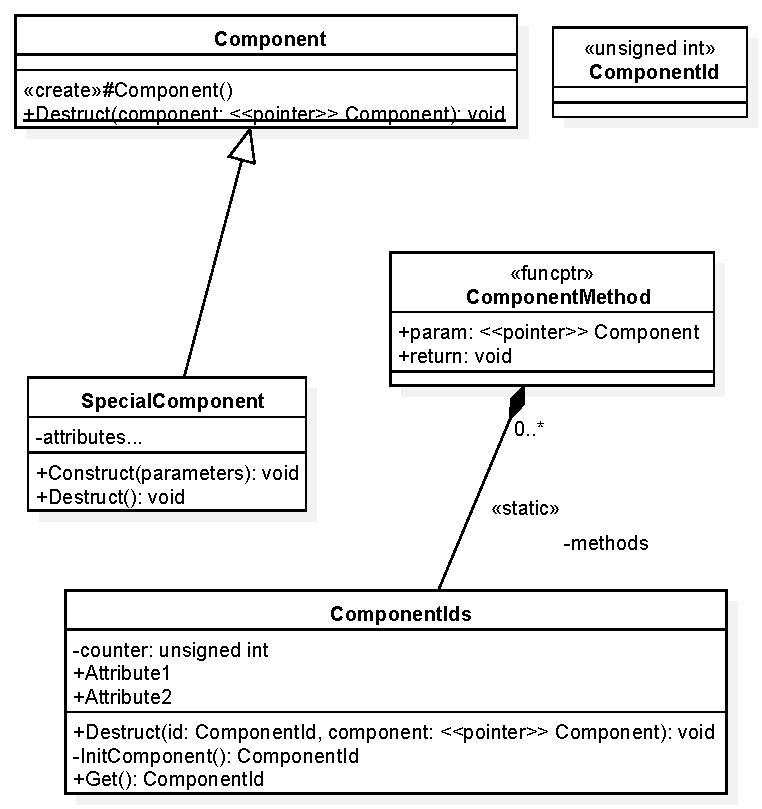
\includegraphics[width=\textwidth]{03unserprogramm/Engine/SpecialComponent.pdf}
		Die Klasse SpecialComponent ist eine Beispiel-Klasse für einen benutzererstellten Komponenten. Hierbei ist attributes für tatsächliche Variablen auszutauschen und parameters für die Parameter, die der Komponent benötigt um initialisiert zu werden. Es können gegebenenfalls auch mehrere Überladungen der Construct-Methode erstellt werden.
		\caption{Klassendiagramm der Component-Klassen}\label{ClassDiagramComponents}
	\end{center}
\end{figure}

Möchte man eine neue Komponente erstellen, so muss man eine Klasse erstellen, die von der Klasse Component erbt. Die Component-Klasse ist eine leere Klasse und dient nur dazu, verschiedene Komponenten auf eine allgemeine Weise zu speichern. 
\todo[inline]{KOMISCHER SATZ: START}
Wenn eine neue Komponente erstellt wird nicht unbedingt der Konstruktor aufgerufen wird, wenn ein alter Komponent wieder verwendet werden kann, muss jede Klasse, die von Component erbt die Methode Construct mit beliebigen Parametern enthalten, sowie die Methode Destruct ohne Parameter. 
\todo[inline]{KOMISCHER SATZ: ENDE}
Da Vererbung in diesem Fall einen großen Geschwindigkeitsverlust bewirken würde, muss die \textit{Construct}-Methode mit Hilfe von Templates aufgerufen werden. Bei der \textit{Destruct}-Methode ist dies leider nicht so einfach möglich, da der Datentyp zum Zeitpunkt der Zerstörung nicht mehr bekannt ist muss ein Funktions-Pointer für jeden Komponenten-Typ gespeichert werden. Dieser zeigt auf eine Funktion, welche einen \textit{Component}-Pointer erst zu dem spezifischen Komponenten-Pointer casted und dann die Destruct-Methode aufruft. Diese Funktion ist eine statische Template-Methode in der Component-Klasse. Mit dem Template-Parameter ist es möglich diese Methode für verschiedene Komponenten zu verwenden. Der Pointer wird in einem Objekt der Klasse \textit{EntityIds} gespeichert und kann verwendet werden, indem die statische Methode \textit{Destruct} aufgerufen wird, der sowohl die Komponente, als auch die ID übergeben wird. 
Er wird beim erstmaligen aufrufen der Methode Get() für jeden Komponent-Typ mit der Methode InitComponent() erstellt. Diese Klassen sind in \cref{ClassDiagramComponents} dargestellt.

Ein Manager ist eine Klasse, die von der Basisklasse \textit{Manager} erbt. 
\todo[inline]{Erklärung des Managers}
\subsection{Window-System}

\subsubsection{Fenster}
Ein Spiel \textit{"`passiert"'} in unserem heutigen Zeitalter wie jedes andere GUI in einem \textit{Fenster}. Um ein solches zu erstellen, wurden in der FM3D-Engine die Klassen \textit{Window} und \textit{Win32Window} implementiert.
Window ist die Basisklasse, von welcher alle Fenster-Typen erben sollen.
Die Klasse besitzt die Attribute \textit{width} und \textit{heigth} vom Typ Integer, welche die Breite und Höhe eines Fensters darstellen.
Es existieren ein Konstruktor und verschiedene Methoden, die die Interaktion mit einem Fenster ermöglichen. Alles erwähnte ist \textit{protected}.
\textit{Start} startet unter Angabe der Parameter, welche die Breite, Höhe, den Fenster Titel, und die Sichtbarkeit des Fensters angeben, das bereits erstellte Fenster.
Die Methode \textit{HasMessage} gibt an ob das Fenster eine Message hat. Shouldclose gibt zurück, ob das Fenster geschlossen werden soll.
Die Methode \textit{Close()} schließt ein Fenster. Mit der Methode \textit{Create()} erstellt man ein neues Fenster mit den Übergabeparametern der Plattform, auf welcher das Spiel bzw. die GUI laufen soll und einem Objekt der Klasse HINSTANCE, welches ein Handle für Windows-Anwendungen ist. Die Methode \textit{StartConsole()} startet eine Konsole für eventuelle Fehlerdiagnosen oder ähnlichem. Mit der Methode \textit{SetConsolePosition} kann man mit Übergabeparametern X und Y vom Typ Integer, die die Koordinaten auf dem Bildschirm beschreiben, die Position der Konsole auf dem Bildschirm setzen.
Jedes Window-Objekt besitzt ein Objekt der Klasse Input, doch dazu später mehr. Die Basisklasse \textit{Window} hat den Vorteil, dass man verschiedene Fensterklassen für verschiedene Betriebssysteme implementieren könnte. In der aktuellen Version der Engine existiert nur eine Fensterklasse für Windows32 die von \textit{Window} erbt. Dies ist die Klasse \textit{Win32Window}. Die Klasse Windows besitzt zudem noch einige \textit{Get-} und \textit{Set-}Methoden, wie Größe und Position des Fensters auf dem Bildschirm.

Wie schon erwähnt, erbt die Klasse \textit{Windows32Window} von der Klasse \textit{Window} und die Klasse \textit{Window} steht zu \textit{Win32Window} in einer \textit{friend} Beziehung.
\textit{Win32Window} besitzt die Attribute \textit{msg} vom Typ \textit{MSG}, \textit{hWnd} vom Typ \textit{HWND}, \textit{hInstance} vom Typ \textit{HINSTANCE} und einen String der den Namen des Fensters beschreibt.
HWND ist ein Windows-Handle für Fenster und \textit{MSG} ein Windows-Datentyp für Informationen über die Nachrichten eines Threads. 
Die Klasse besitzt zudem einen Konstruktor, dem man ein Objekt der Klasse \textit{HINSTANCE} übergibt, vier \textit{public} Methoden und eine \textit{private} Methode. Die Methode \textit{Start} startet das Fenster und benötigt als Übergabeparameter die Höhe, die Breite, den Titel des Fensters und einen boolschen Wert, der angibt, ob das Fenster angezeigt werden soll, oder nicht.
Auch hier gibt die Methode HasMessage an, ob das Fenster eine Message hat und Shouldclose gibt zurück, ob das Fenster geschlossen werden soll. Nur sind diese Methoden auf Windows32 zugeschnitten und verwenden unteranderem auch die Methoden aus der Klasse Window.
\textit{Close} schließt das Fenster. (für weitere Informationen Siehe \cref{Windowsystem})

\begin{figure}
	\begin{center}
		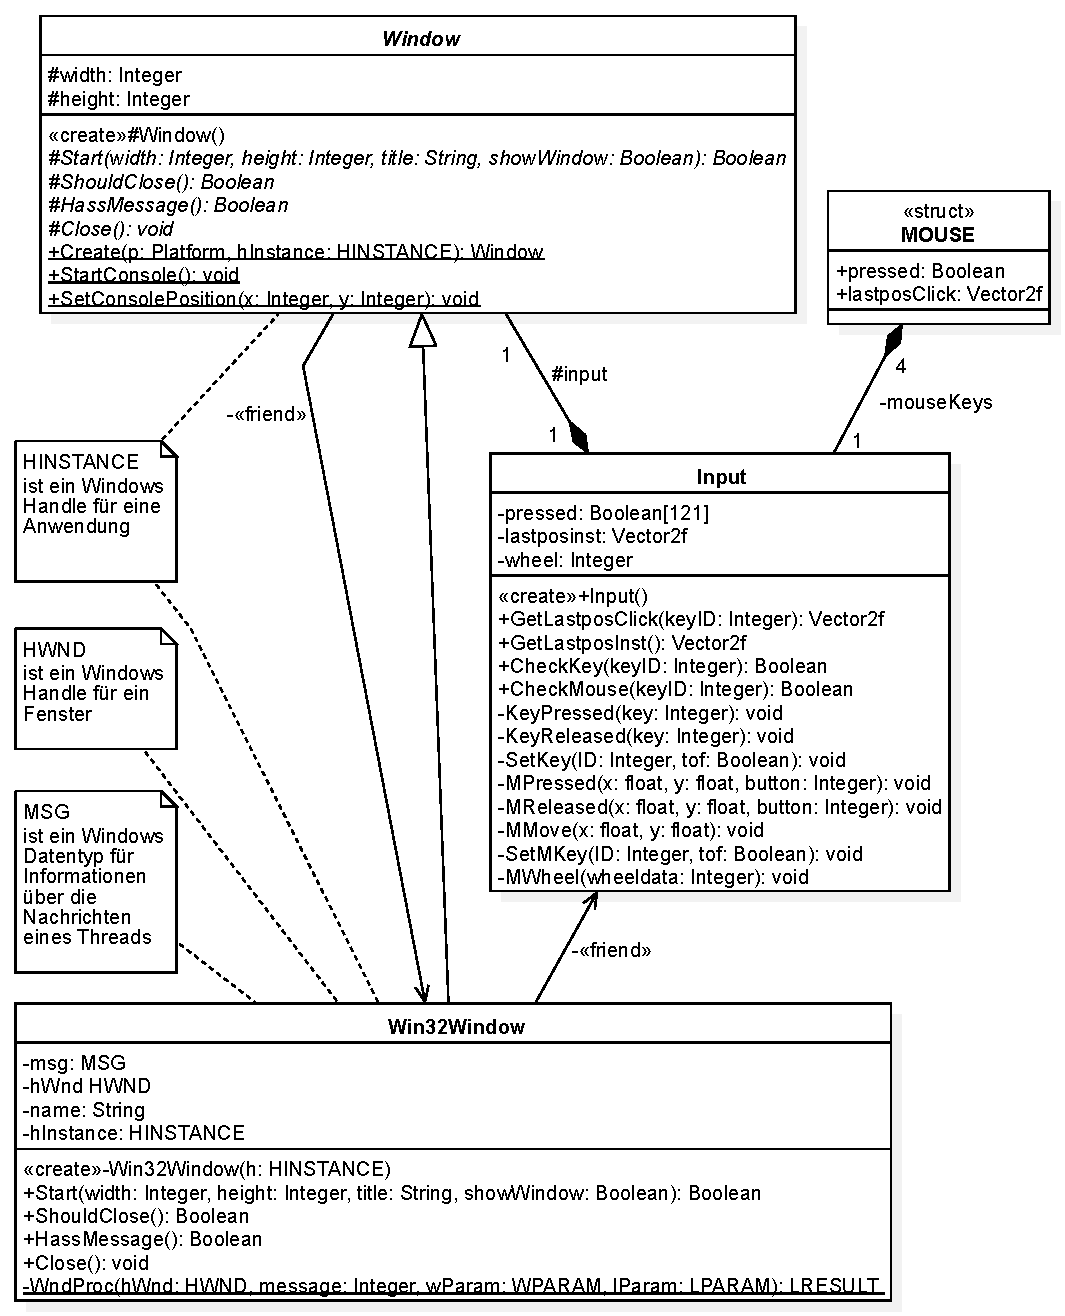
\includegraphics[width=\textwidth]{03unserprogramm/Engine/WindowSystem.pdf}
		Es wurde auf die Angabe von Get- und Set-Methoden sowie Events verzichtet.
		\caption{Window-System}\label{Windowsystem}
	\end{center}
\end{figure}

\subsubsection{Input-Klasse}

Natürlich benötigt ein Spiel bzw. auch die meisten grafischen Nutzer-Oberflächen auch ein sicheres Eingabe-System, welches sowohl die Position der Maus ermittelt, aber auch die Abfrage jeder einzelnen Taste auf der Tastatur regelt. 
Dafür wurde in der FM3D-Engine eine eigene Klasse implementiert, welche für diesen Aufgabenbereich zuständig ist.
Um den Nutzer der FM3D-Engine davor zu bewahren, nicht jeden einzelnen ASCII-Code jeder Taste auf der Tastatur nachzuschlagen, sind alle Tasten in Form von Makros definiert. 
In dem Namespace FM3D befindet sich die Klasse \textit{Input} und jedes Objekt eines Fensters bzw. der Klasse \textit{Window} besitzt ein Objekt dieser Klasse. Die Klasse \textit{Input} beinhaltet außerdem die Enumeration \textit{KEYCLICK}, welches den aktuellen Zustand der Maustasten beschreibt. Diese können entweder gedrückt, nicht gedrückt oder losgelassen werden und sind in dieser Enumeration definiert.
Eine Struktur \textit{MOUSE} enthält die Enumeration \textit{KEYCLICK} und einen zweidimensionalen Vektor des Typen \textit{Float}, welcher die zweidimensionale Position im Fenster in OpenGL Koordinaten angibt, an welcher eine Taste der Maus gedrückt wurde.
Diese Struktur wird in der Klasse Input als ein vier-Felder Array verwendet, welches jede Taste einer durchschnittlichen Maus beschreibt. Diese sind die linke, die rechte und die mittlere Maustaste. Das letzte Feld ist für ein zusätzliches Feld einer beliebigen Taste der Maus reserviert, da es immer unterschiedliche Maus-Typen gibt.
Zudem besitzt die Klasse \textit{Input} einen Vektor \textit{lastposinst}, welcher ununterbrochen die Position der Maus ermittelt. Dies ist in den Spielen erforderlich in denen die Maus ununterbrochen die Kamera steuert.

Für die Tastenabfrage wurde zunächst ein Integer Wert verwendet, in welchen der aktuell gedrückte ASCII-Code gespeichert wurde. Dies hat aber den Nachteil, dass nur eine Taste gedrückt sein bzw. abgefragt werden darf. Möchte man nun zum Beispiel einen Spiele-Charakter schräg durch einen Raum mit gedrückter Links- \textbf{und} Rechts-Taste bewegen, so wäre hiermit nicht möglich. Deswegen beschreibt nun ein 121-Felder Array aus booleschen Werten die komplette Tastatur. Jede Feldnummer ist äquivalent zu dem zugeordneten ASCII-Code der Taste. Die Felder [1] bis [4] beschreiben die Maustasten. Einige Felder des Arrays sind nicht von einem ASCII Code auf der Tastatur \textit{belegt} und sind somit "`\textit{frei}"'. Dies hat den Vorteil, dass später simpel weitere Eingabegeräte in die Klasse Input eingebunden werden können.
Die Klasse besitzt Methoden, welche in der Klasse Win32Window.h (Siehe Doxygen Dokumentation), die ein GUI-Fenster abbildet, die die verschiedenen Werte der Arrays und des Vektors setzen.
Zudem besitzt die Klasse Methoden, die diese Werte zurück geben. (Für die Verwendung dieser Klasse siehe \cref{inputsystemver})



\section{Engine - Allgemeiner Aufbau}

Die Engine ist eine Visual C++ Laufzeitbibliothek (Dynamic-Link-Library; DLL). Diese DLL enthält den gesamten Code, welcher zum Erstellen eines Spieles erforderlich ist. Jason Gregory beschreibt in seinem Buch den Aufbau einer Game-Engine als eine Struktur aus Systemen und Schichten. 
Hierbei können mehrere Schichten übereinander liegen. Ideal verwenden die höher gelegenen Schichten bereitgestellte Funktionalitäten der unteren Schichten, was aber nie umgekehrt geschehen soll. Dies ermöglicht die Abschirmung von hardwareabhängigen und spielnahen Klassen. Ein System übernimmt eine bestimmte Aufgabe und kann sich über mehrere Schichten ausbreiten. \cite{gea}
Die FM3D-Klasse hat diese Idee in bestimmten Teilen übernommen. Im Code ist die System-Struktur als Ordner-Struktur wiederzufinden. Diese Systeme sind teilweise auch durch einen \textit{Namespace} oder Präfix vor jedem Namen zu erkennen. Das Schichtenmodell ist in der Engine als mehrere Untersysteme (auch Subsystems genannt) erkennbar. Diese Untersysteme sind genauso zu erkennen und verhalten sich wie normale Systeme. Der einzige Unterschied ist, dass sie sich bereits in einem System befinden.

\section{Engine - Allgemeiner Aufbau}

Die Engine ist eine Visual C++ Laufzeitbibliothek (Dynamic-Link-Library; DLL). Diese DLL enthält den gesamten Code, welcher zum Erstellen eines Spieles erforderlich ist. Jason Gregory beschreibt in seinem Buch den Aufbau einer Game-Engine als eine Struktur aus Systemen und Schichten. 
Hierbei können mehrere Schichten übereinander liegen. Ideal verwenden die höher gelegenen Schichten bereitgestellte Funktionalitäten der unteren Schichten, was aber nie umgekehrt geschehen soll. Dies ermöglicht die Abschirmung von hardwareabhängigen und spielnahen Klassen. Ein System übernimmt eine bestimmte Aufgabe und kann sich über mehrere Schichten ausbreiten. \cite{gea}
Die FM3D-Klasse hat diese Idee in bestimmten Teilen übernommen. Im Code ist die System-Struktur als Ordner-Struktur wiederzufinden. Diese Systeme sind teilweise auch durch einen \textit{Namespace} oder Präfix vor jedem Namen zu erkennen. Das Schichtenmodell ist in der Engine als mehrere Untersysteme (auch Subsystems genannt) erkennbar. Diese Untersysteme sind genauso zu erkennen und verhalten sich wie normale Systeme. Der einzige Unterschied ist, dass sie sich bereits in einem System befinden.
\section{GUI-Fenster}
\label{guifenster0}

(Zum besseren Verständnis siehe \cref{windowclass})
Der Designer verfügt im allgemeinen drei Typen wie Seiten der GUI dargestellt werden können: Das Programm besitzt ein Hauptfenster, welches das Design von MahApps.Metro verwendet. (Siehe \cref{mahapps})
Dieses Hauptfenster kann nun in verschiedene Reiter unterteilt werden. Dies gehen wir mit der GUI Bibliothek DotNetBar (Siehe \cref{dotnetbar}) an.
Diese Reiter sind im Designer sogenannte \textit{Layouts}. Jeder der verschiedenen Layoutklassen stehen im Namespace \textit{FM3D\_Designer.src.WindowLayouts} und erben von der Klasse \textit{WindowLayout} im Namespace \textit{FM3D\_Designer.src}. Diese Klasse beinhaltet Attribute die jedes der Layouts verfügt. Die Klasse WindowLayout, welche wiederum von der Klasse \textit{DockWindow} der DotNetBar-Bibliothek erbt, sorgt dafür, dass die verschiedenen Seiten als Reiter und Unterfenster (oder auch child-windows) behandelt werden.
In jedem Layout ist es möglich verschiedene  kleinere Fenster aufzurufen. Der User kann diese Fenster innerhalb der Layouts oder des Desktops andocken. Jedes dieser \textit{ToolWindows} ist der Strukturierung wegen nochmal in einen weiteren Namespace unterteilt. Alle dieser \textit{ToolWindows} erben von der Klasse \textit{ToolWindow}, welche eine Initialisierungsmethode und eine Aggregation zu einem \textit{WindowLayout} verfügt.
Auch die Klasse \textit{ToolWindow} erbt von der Klasse \textit{DockWindows}.
Neben diesen Reitern und Unterfenstern verwendet der Designer noch sogenannte \textit{Dialoge}. All diese Dialoge erben von der Klasse \textit{DialogBase}, welche die Grundkomponenten der Dialoge beinhaltet. Diese Klasse erbt wiederum von \textit{BaseMetroDialog} welche sich in der MahApps.Metro Bibliothek befindet. 

\begin{figure}
	\begin{center}
		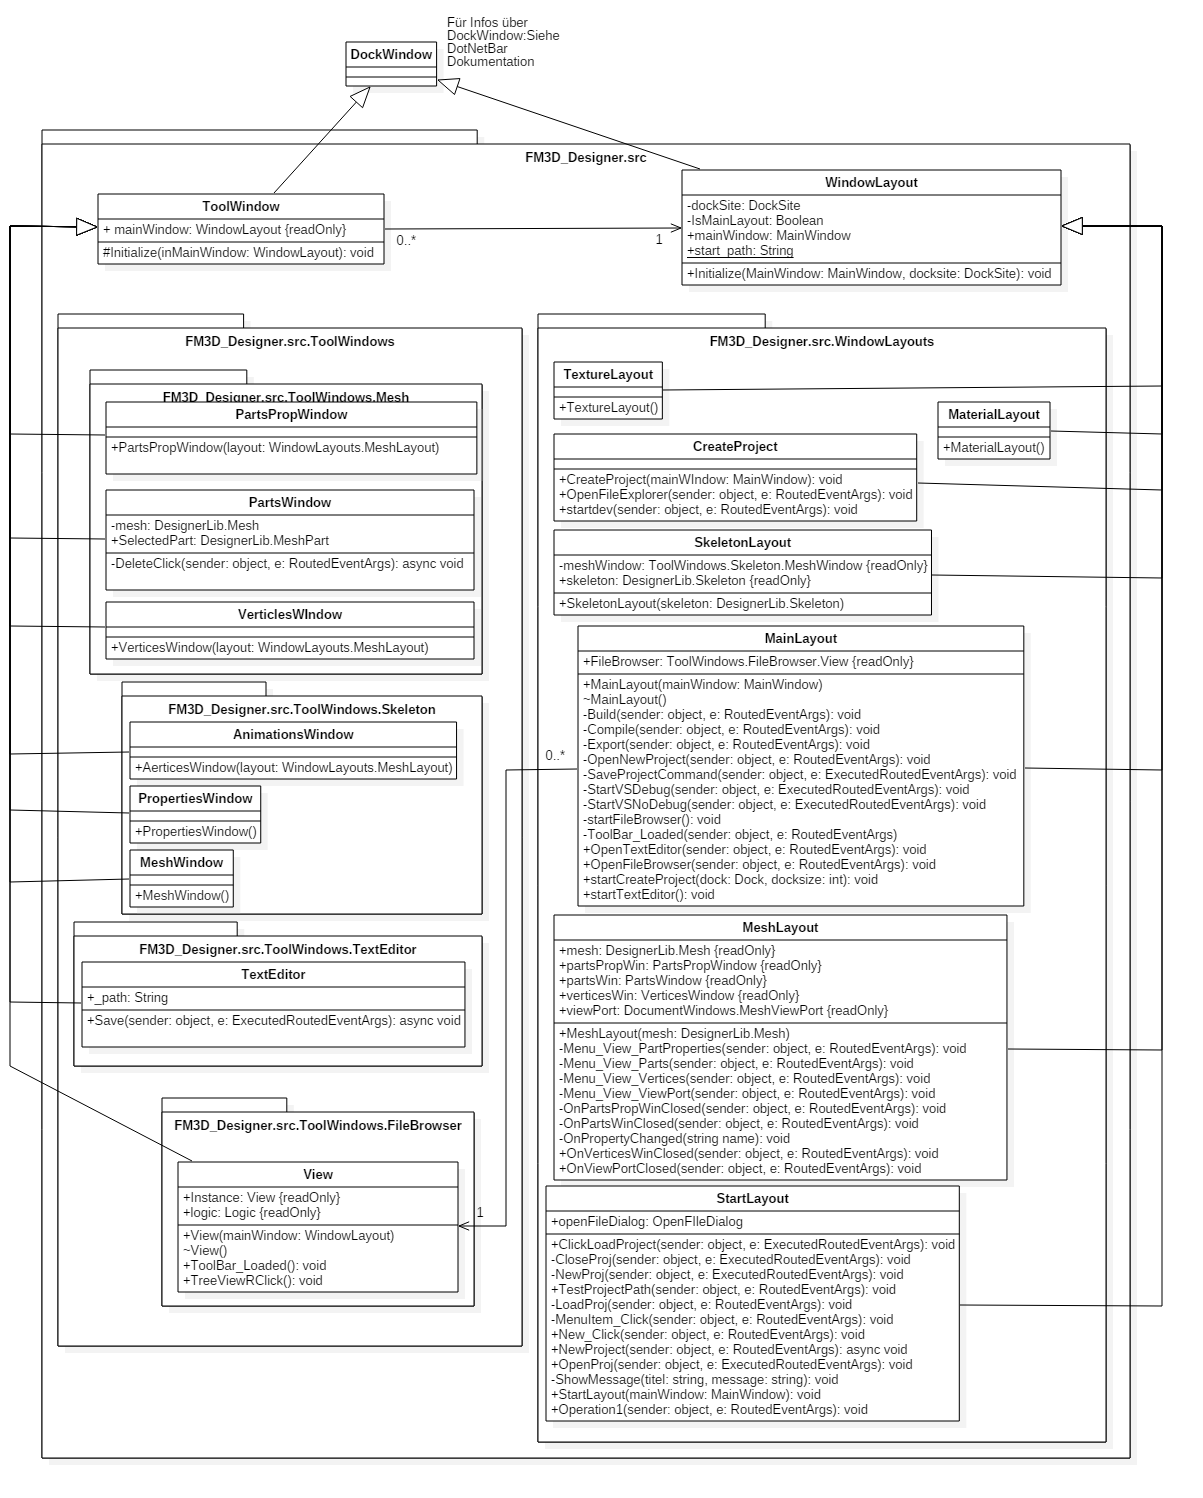
\includegraphics[width=1.2\textwidth]{03unserprogramm/Designer/Layouts.png}
		\caption{Fenster-Klassen}\label{windowclass}
	\end{center}
\end{figure}

\begin{figure}
	\begin{center}
		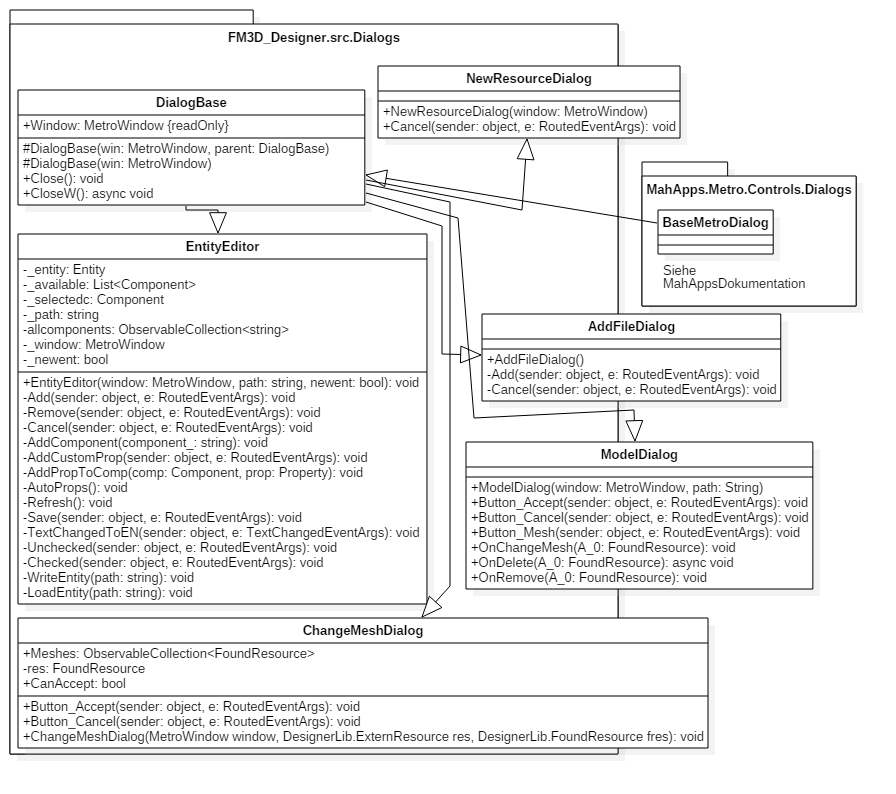
\includegraphics[width=\textwidth]{03unserprogramm/Designer/Dialogs.png}
		\caption{Dialog-Klassen}\label{dialogclass}
	\end{center}
\end{figure}

\subsection{Layouts}
\subsubsection{StartLayout}
\label{startlayout}
Das Start-Layout des Designers bietet dem Nutzer die Option ein Projekt in den Designer zu laden oder ein neues zu erstellen. Möchte man nun eines erzeugen, so wird man auf einen neuen Reiter gewiesen, in dem man nun Einstellungen bezüglich des zu erstellenden Projektes tätigen kann. Rechts davon befindet sich ein Text mit einem kurzen Anweisungstext zu dem Programm. Darunter ist ein Internet-Browser eingebunden, welcher die letzten Änderungen des Programmes anzeigt.

\subsubsection{CreateProjekt}
Nachdem man auf einen Nebenreiter des Startlayouts geleitet wurde, kann der User einen Pfad bestimmen in dem das Projekt geladen werden soll. Im vom User angegebenen Pfad werden jetzt zwei Ordner angelegt: Einen für die Projektdateien und einen für die C++ Dateien. 
In den Ordner der C++ Dateien wird nun ein VisualStudio-Projekt-Template erstellt, welches ein Projekt für das Spiel abbildet. Zu diesem wird eine "'fm3D.xml"` Datei in dem selben Ordner generiert. In dieser stehen Informationen, welche später für die Pipe \ref{pipe} benötigt werden. Darunter der Dateiname, Der Projektmappenname und die Pipe-ID.
Nun wird die Projektdatei in Form von einer XML-Datei mit der Endung "'.fmproj"` erzeugt. Diese wird beim Start der FM3D-Designer-Entwicklungsumgebung geladen und später in der \textit{TreeView} des \textit{File-Browsers} dargestellt.

\subsubsection{MainLayout}
\label{mainlayout}
Nachdem nun ein Projekt erstellt oder geöffnet und geladen wurde, wird der User auf das "'Main-Layout"` geleitet. Dort werden mit dem Start ein Texteditor und ein File-Browser in andockbaren Childfenstern geöffnet. In dem Kontextmenü des Programmes kann der User nun zwischen vier verschiedenen Reitern auswählen. Neben jeder Option werden zudem -falls Verfügbar- Tastenkürzel angezeigt. 
In dem ersten Reiter "'File"` kann der User entweder ein neues Projekt erstellen oder das aktuelle speichern. 
Im zweiten Kontextmenüitem sind die Operationen aufrufbar, welche für die Kommunikation mit der Extension (\ref{extension}) über die Pipe(\ref{pipe}) benötigt werden. Diese Optionen sind auch in Icons unter dem Kontextmenü abgebildet, um dem User ein schnelles arbeiten zu ermöglichen. Im dritten Kontextmenüitem kann man nun die verschiedenen andockbaren Fenster auswählen. Im vierten und letzten sind Informationen zum Entwicklerteam und über dieses Projekt zu finden.

\subsubsection{MeshLayout}
Das MeshLayout wird verwendet um ein geöffnetes Mesh anzuzeigen. Dabei verwendetet es eine einfache Menüleiste, die es erlaubt verschiedene Toolwindows zu öffnen oder in den Vordergrund zu hohlen und das geladene Mesh zu speichern. Im MeshLayout ist das Mesh gespeichert und die Mesh-Toolwindows greifen über diese Klasse darauf zu, genauso wie auf andere Toolwindows. Zum Speichern werden die Methoden der DesignerLib verwendet.

\subsection{ToolWindows}
\subsubsection{FileBrowser}
\label{filebrowser}
Im File-Browser wird die Ordnerstruktur des FM3D-Projektes in Form der \textit{Item}-Klasse (Siehe \cref{item}) abgebildet. Der Nutzer kann durch diesen File-Browser nun entweder Daten erstellen oder sich diese darstellen lassen. Entity-Dateien können durch den Entity-Editor grafisch betrachtet und editiert werden. Alle abgebildeten Dateien können zudem in einem im Designer implementierten Text-Editor mit den nötigsten Funktionen bearbeitet werden.

\subsubsection{TextEditor}
Der Texteditor ist ein Tool um Texte zu editieren.  Es verfügt über die wichtigsten Funktionen, die ein Text-Editor verfügen sollte. Jede dieser Funktionen sind über Tastenkürzel aufrufbar.
\begin{itemize}
	\item Speichern
	\item Undo/Redo (Rückgängig/Wiederherstellen)
	\item Copy/Cut (Kopieren/Ausschneiden)
	\item Paste (Einfügen)
	\item Delete (Löschen)
\end{itemize}

\subsubsection{Mesh-Parts-Window}
Ein Mesh besteht aus mehreren Parts, welche alle in einer Listbox angezeigt werden. Andere Toolwindows verwenden dieses um herauszufinden welches Parts ausgewählt ist und demnach genauere Informationen zu zeigen. Wenn ein neuer Part ausgewählt wird updaten sich automatisch alle anderen Windows durch die Verwendung des \textit{INotifyPropertyChanged-Interface}. Es ist möglich mit einem Rechtsklick ein Part zu löschen, umzubenennen oder auszublenden.

\subsubsection{Mesh-Vertices-Window}
In diesem Fenster werden in einer Tabelle alle Vertices des aktuell ausgewähltenb Mesh-Parts angezeigt. Dafür müssen alle Vertices in Strings umgewandelt werden, was sehr Zeit aufwendig ist und viel Speicher verbraucht, daher ist es empfohlen dieses Toolwindow nur für kleinere Parts zu verwenden. 

\subsubsection{Mesh-Parts-Property-Window}
Dieses Toolwindow zeigt alle Eigenschaften eines Mesh-Parts. Zum Anzeigen wird ein PropertyGrid aus der DotNetBar-Bibliothek genutzt, da dieses automatisch alle Properties eines Objektes in die Tabelle einträgt. Um auszuwählen welche Properties angezeigt werden sollen und mit welcher Beschreibung besitzen alle Properties der Designerlib.MeshPart-Klasse dafür zuständige Attribute.

\subsubsection{Skeleton-Tools}
\todo[inline]{idk}

\subsection{Dialogs}
\subsubsection{Model-Loader | Add Resource-Dialog}
Der Model-Loader ist dafür gedacht, um simpel Modelle in den Designer zu laden, um sie dann in der Engine weiter verwenden zu können. Die Modeldatei wird analysiert und die Daten werden in eine Datei in der Ordnerstruktur des Designers gespeichert.
%Durch die Exportfunktion im Designer kann man nun Code generieren lassen, der die Modelle im Designer verwenden kann 
\todo[inline]{!!!}

\subsubsection{Entity-Editor}
\label{entityeditor}
Der Entity-Editor wurde implementiert, um dem Nutzer das erstellen von Entities zu erleichtern. (Um den Aufbau der Entities erfahren siehe: \ref{entitysystem}). Der Nutzer gibt im Entity-Editor zunächst die Komponenten ein, die das zu erstellende Entity haben soll. Zu diesen Komponenten werden nun optional Standart-Properties bereitgestellt, die automatisch hinzugefügt werden können. Der User kann außerdem noch weitere, Benutzer spezifische Properties zu den Entities hinzufügen. Diese ganzen Daten werden nun in Form einer .xml Datei mit der Endung "'.ent"` im Projektordner gespeichert. Diese kann sich der Nutzer sowohl mit einem externen oder mit dem implementierten Texteditor im FM3D-Designer anschauen und wenn es ihm beliebt manuell verändern.



\section{Logik}
Neben den Klassen, in denen die Fenster beschrieben werden, existieren auch Klassen in denen die Logik beschrieben steht. Diese werden in diesem Unterkapitel behandelt.

\subsubsection{Project-Klasse}
Die \textit{Project}-Klasse stellt ein FM3D-Projekt dar. Es besitzt Methoden, um Projekte aus \ac{XML}-Dateien zu laden, in \ac{XML}-Dateien zu speichern und den Projektnamen zu setzen. Zudem besitzt es eine Instanz zu dem gerade aktiven Projekt und den Projektnamen und das Verzeichnis in Form des Datentyps \textit{String}. Auf die Unterverzeichnisse kann man durch ein Objekt der \textit{RootDirectory}-Klasse\cref{rootdirectory} zugreifen.

\subsubsection{RootDirectory-Klasse}
\label{rootdirectory}
Diese Klasse erbt von der Klasse \textit{Directory} (Siehe \cref{directory}) und stellt das sogenannte Wurzelverzeichnis dar. Sie besitzt ein Boolean, mit dem dargestellt wird, ob das Verzeichnis im FileBrowser (Siehe \cref{filebrowser}) angezeigt werden kann.

\subsubsection{Directory-Klasse}
\label{directory}
Die \textit{Diretory}-Klasse besitzt drei \textit{ObservableCollections} in Form von Objekten der Klassen \textit{FileObject}, \textit{File} und \textit{Directory}. Dadurch dass die Directory-Klasse \textit{ObservableCollections} des eigenen Types hat, kann eine simple Baumstruktur von Ordner gebildet werden. Sie erbt von der \textit{FileObject}-Klasse. \cref{fileobject}

\subsubsection{File-Klasse}
Diese Klasse erbt auch von der \textit{FileObject}-Klasse. Sie wird in der \textit{Directory}-Klasse verwendet um die Projektdateien zu beschreiben.

\subsubsection{FileObject-Klasse}
\label{fileobject}
Diese Klasse beschreibt die Grundstruktur eines Objektes, welches in einer Ordnerstruktur bzw. in einem FM3D-Projekt dargestellt wird. Der Dateiname und Dateipfad werden durch den Datentyp String beschrieben.

\subsubsection{Filebrowser View-Logic}
\label{fbview}
Die Klasse \textit{Logic}, welche im Namespace "`\textit{FM3D\_Designer.src.ToolWindows.FileBrowser}"' steht, erbt von dem Interface \textit{INotifyPropertyChanged}. \textit{INotifyPropertyChanged} ist ein Interface, womit Events gefeuert werden können, wenn sich eine bestimmte Eigenschaft ändert, sodass andere Klassen wie zb. ein Fenster darauf reagieren können.
Dies benutzt man hier, um \todo{!!!}
Die Klasse enthält eine Enumeration, welche die Anzeigeeinstellung des File-Browser beschreibt. 
Eine in der Klasse \textit{Logic} stehende \textit{ObservableCollection} enthält alle Wurzelverzeichnisse, welche mit der Klasse \textit{Item} beschrieben werden. In einem Objekt der Klasse \textit{Item} namens \textit{\_CurrentDirectory} und der Eigenschaft \textit{CurrentDirectory}, welche das \textit{Item}-Objekt von \textit{\_CurrentDirectory} zurück gibt, wird das aktuelle . Ein Interface vom Typ \textit{IList} gibt den Inhalt der aktuell ausgewählten \textit{Directory} im File-Browser (Siehe \cref{filebrowser}) zurück. Zudem besitzt diese Klasse verschiedene Methoden zur Interaktion mit dem File-Browser.

\subsubsection{Item}
\label{item}
Objekte der Klasse \textit{Item} sind dafür , im \textit{File-Browser} angezeigt zu werden. Die Klasse erbt von dem Interface \textit{INotifyPropertyChanged}, welches schon in \cref{fbview} erläutert wurde. Ein \textit{Item} besitzt eine Enumeration namens \textit{ItemState}, welche angibt, ob das Item im Projekt eingebunden, nicht eingebunden wurde oder nicht in der Ordnerstruktur gefunden wird. Es besitzt zudem ein Objekt der Klasse ItemType, um den Typ der Datei anzugeben, und ein Objekt der Klasse Logic. So kann auch hier, ähnlich wie bei der Klasse \textit{Directory}, eine Baumstruktur gebildet werden.
%%  Dictionary<ItemType, List<Item>>
Ein rekursives Objekt der Klasse Item gibt das \textit{Parent}-Item an. Dies ist das \textit{Item}, welches das übergeordnete Verzeichnis angibt.
Ein Item besitzt zudem ein \textit{ContextMenu}, welches bei einem Rechtsklick auf das Item geöffnet wird. Des weiteren wurden Methoden Implementiert, welche verschiedene Dialoge und Fenster öffnen. Man kann durch sie den \textit{Text-Editor}, den \textit{Entity-Editor} und den \textit{AddNewResource}-Dialog öffnen, welche sofort mit diesem \textit{Item} interagieren.
Die Methode \textit{CreateFile} kann mit Angabe eines Dateinamen, einem \textit{ItemType} und dem \textit{Item}, das gerade angeklickt ist, eine neue Datei erstellen. Dies geschieht im Programm über das \textit{ContextMenu} durch den \textit{AddResource}-Dialog.

\subsubsection{ItemType}
Diese Klasse gibt den Typ eines Item an. Sie besitzt einen Container in Form eines \textit{Dictionary}. Als Schlüsselwert/Key wird ein String verwendet. Der Wert/Die Value ist ein Rekursives Objekt der selbigen Klasse \textit{ItemType}.
In ItemType stehen statische einzelne rekursive Objekte der selbigen Klasse für jeden Dateien-Typ den es in dem FM3D-Projekt existiert.
Jeder Typ besitzt Pfade zu den Icons, welche im File-Browser angezeigt werden.  Es existieren insgesamt acht verschiedene:
\begin{itemize}
	\item Directory
	\item UnknownFile
	\item EntityFile
	\item MaterialFile
	\item SkeletonFile
	\item MeshFile
	\item TextureFile
	\item ModelFile
\end{itemize}


\subsubsection{Entity-Klassen}
\label{entityklassen}
Sowohl im Designer als auch in der Extension gibt es jeweils die selben drei Klassen, welche für die Entities zuständig sind: \textit{Entity}, \textit{Component} und \textit{Property}.
Die \textit{Entity} Klasse beschreibt das Entity, so wie sie später im Code erstellt werden sollen. Ein Entity-Objekt besitzt einen Namen und drei Container des Typen \textit{List}. Die erste Liste besitzt Objekte der Klasse \textit{Component}, die zweite und dritte Liste sind Objekte der Klasse \textit{Property} und sind jeweils für die automatisch generierten und für die benutzerdefinierten Properties.
Jeder dieser Klassen besitzt zudem eine überladene \textit{ToString()} Methode, welche dafür sorgt, dass alle Daten in ein String geschrieben werden, um sie dann später per Pipe zu verschicken.
Um die einheitliche Trennung der Daten durch verschiedene \textit{Chars} in diesem zu versendenden Stringdatensatz zu gewährleisten wurde die statische Klasse \textit{SC} implementiert, welche die Trennungszeichen beinhaltet.
Jeder dieser drei Klassen -die statische Klasse \textit{SC} zählt nicht dazu, da sie nur eine Sammlung von Zeichen zur Trennung sind- enthalten noch einen Konstruktor, welcher einen umgewandelten Datensatz vom Typ String wieder in eines dieser Objekte umwandelt. 
So können, nachdem ein Entity in Form eines Datensatzes vom Typ String per Pipe an die VisualStudio-Extension geschickt wurde, die Daten dort weiterverwendet werden. 
Die Klassen werden in \cref{entityklassendiag} dargestellt.
\begin{figure}
	\begin{center}
		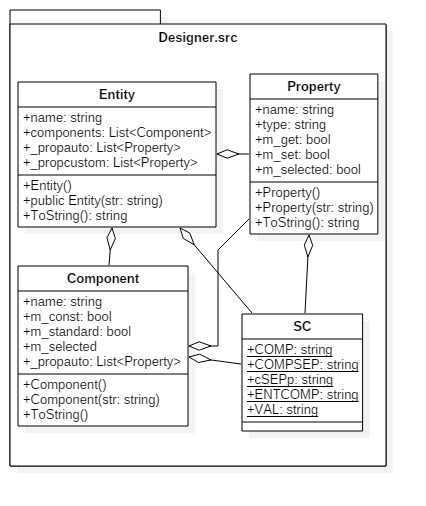
\includegraphics[width=0.4\textwidth]{03unserprogramm/Designer/EntityKlassen.png}
		\caption{Entity-Klassen im Designer}\label{entityklassendiag}
	\end{center}
\end{figure}

\subsubsection{Creator}
Um ein Item zu erstellen muss die Klasse Creator verwendet 
\todo[inline]{!!!}
\subsubsection{FM3DPropertyFile-Klasse}
Diese Klasse ist dafür zuständig, Daten aus der Datei \textit{fm3d.xml} zu lesen. Diese Datei beinhaltet Daten für die Kommunikation mit der Extension per Pipe. Sowohl im Designer als auch in der Extension sind zwei von der Grundstruktur sich ähnelnde Klassen der \textit{FM3DPropertyFile}-Klasse.

\subsubsection{PipeSystem} 
\label{pipe}
Grob betrachtet ist die Pipe eine Klasse, welche die Kommunikation zwischen zwei Programmen ermöglicht. In unserem Fall kommunizieren der FM3D-Designer und die dazugehörige VisualStudio-Extension\ref{extension}. Das ganze läuft relativ ähnlich wie bei simpler Netzwerkkommunikation ab. 
Sowohl im Designer als auch in der Extension sind von der Grundstruktur sich ähnelnde Klassen des PipeSystems.

\subsubsection{FM3D-Extension}
\label{extension}
Die FM3D-Extension ist eine von uns entwickelte Erweiterung für VisualStudio. Sie ist dafür zuständig gesendete Entities\ref{entityklassen} in C++ Code umzuwandeln. In \cref{vsextensiondia} wird der Aufbau der Extension dargestellt.
\begin{figure}
	\begin{center}
		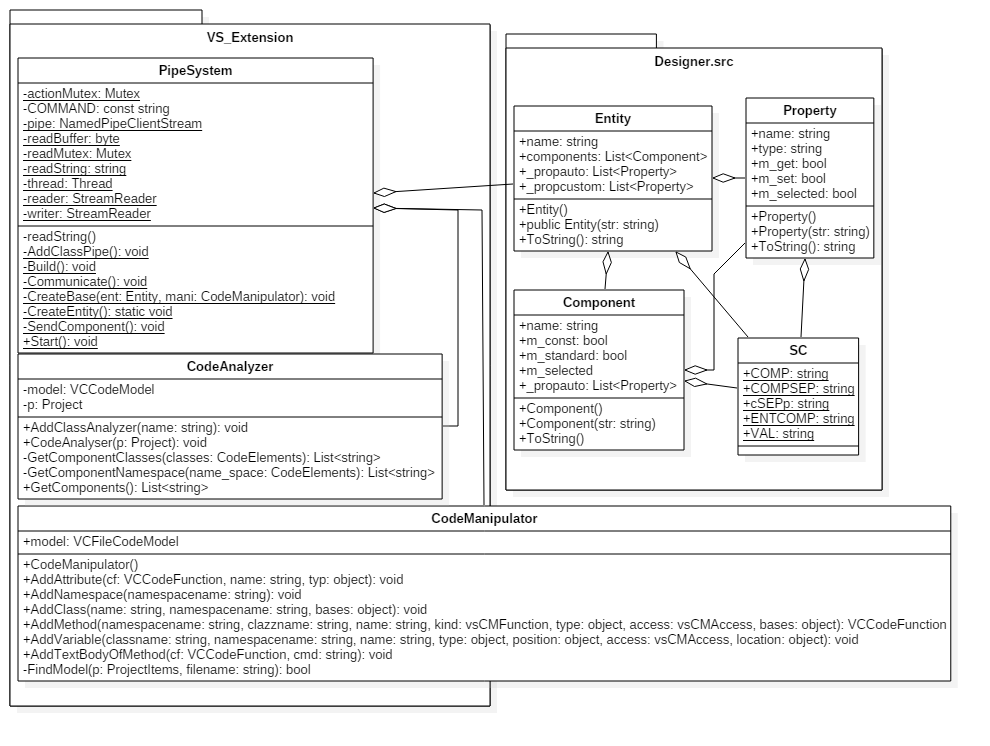
\includegraphics[width=\textwidth]{03unserprogramm/Designer/VSExtension.png}
		\caption{VisualStudio-Extension}\label{vsextensiondia}
	\end{center}
\end{figure}

\section{Externe Bibliotheken}
\subsection{OpenGL}
\label{opengl}
\subsubsection{Beschreibung der OpenGL}
Zum Darstellen von Grafiken wird von der FM3D-Engine OpenGL (Open Graphics Library, deutsch: Offene Grafikbibliothek)verwendet. Diese Bibliothek ist eine Schnittstelle für Grafikanwendungen, die es ermöglicht auf Funktionen der Grafikkarte zugreifen zu können. Geschrieben ist sie in C was ein Problemloses Einbinden in C++ ermöglicht.

Da Grafikkarten immer innovativer werden und somit mehr Leistung bekommen, wird OpenGL immer weiter entwickelt. So entstehen immer wieder neuere Versionen der Bibliothek. Die aktuellste Version ist OpenGL 4.5 (Stand 2016). 

Die verschiedenen Versionen werden grundsätzlich in zwei Gruppen unterteilen: \textit{Legacy OpenGL} und \textit{Modern OpenGL}. \textit{Modern OpenGL} beschreibt hier alle Versionen ab 3.0. und \textit{Legacy OpenGL} alle Versionen darunter. 

Die FM3D-Engine verwendet ausschließlich modern OpenGL 3.3. und höher. Dies bietet weit aus mehr Flexibilität und bessere Performance. Eine frühere Version von OpenGL wäre obsolet.
Rechner dessen Grafikkarte höchstens \textit{Legacy OpenGL} verwenden, wären nicht im Stande modernes 3D-Rendering zu unterstützen.

Hier zu erwähnen sind auch die Erweiterungen von OpenGL. Da OpenGL nicht nur von einer einzigen Firma entwickelt wird, sondern viele Firmen ein Mitspracherecht haben, werden neue Funktionen meist speziell von einem Hersteller entwickelt. Funktionen dieser Erweiterungen erhalten einem zum Hersteller gehörenden Suffix. Wenn sich mehrere Hersteller zusammenschließen für eine Erweiterung bekommt sie den Suffix „EXT“. Wenn das Architecture Review Board ARB beschließt eine Erweiterung hinzuzufügen, so bekommt sie den Suffix „ARB“ und wird in der nächsten Version zum Core-Library hinzugefügt. 

In der FM3D-Engine wird versucht diese Erweiterungen möglichst zu vermeiden. Hersteller spezifische Erweiterungen werden gar nicht verwendet, damit die Engine auf möglichst vielen Systemen verwendet werden kann. Leider sind einige der für die FM3D-Engine wichtigen Funktionen die verwendet werden noch nicht in der Core-Library. Daher müssen Erweiterungen verwendet werden.

\subsubsection{Funktionsweise}

Mit OpenGL kann man nicht direkt zB. einen Delphin oder einen Baum rendern. Da OpenGL nur Dreiecke  rendert, benötigt man um diese Abbildungen darzustellen ein 3D-Modell. Dieses besteht aus Dreieckigen flächen die aus "Verticles" (Punkte) gebildet werden. (Siehe \cref{Dolphin})

Neben den Dreiecken ist es zudem möglich einzelne Linien oder Punkte zu rendern. Dies Folgt dem gleichen Prinzip, nur werden hierbei weitaus weniger Punkte zur eindeutigen Definition benötigt. Dies ist aber bei der Darstellung von den 3D-Modellen nicht wirklich relevant. 
Möchte man also nun einen Delphin darstellen, so braucht man ein 3D-Modell, welches einen Delphin darstellt und aus den besagten Dreiecken besteht. Solche Modelle kann man mit verschiedenen Modellierungsprogrammen wie zum Beispiel "Blender" oder "3DS-MAX" erstellen.

Früher nutzte OpenGL eine Fixed \textit{function pipeline}. Damit war gemeint, dass fest in der Grafikkarte definiert war, wie die Dreiecke verarbeitet und gerendert werden. Man konnte jedem Punkt des Dreiecks einen feste Koordinate %Punkt
zuweisen und optionale weitere Attribute wie Textur-Koordinaten und Farbe hinzufügen. Mit diesen Werten wurde das Dreieck dann gerendert. Heute gibt es sogenannte \textit{Shader}. Diese bestimmen wie ein Objekt gerendert wird. 
\subsection{Windows Presentation Foundation}
\label{wpf}

Windows Presentation Foundation \ac{WPF} ist eine 2006 eingeführte Bibliothek. \cite{wikipedia_wpf} "`Sie vereint die Vorteile von DirectX, Windows Forms, Adobe Flash, HTML und CSS."'\cite{eiwpf} 
Das Aussehen der Anwendungen werden mit der \textit{Extensible Application Markup Language} \ac{XAML} deklarativ beschrieben. Die Logik wird mittels C\# implementiert. So sind Arbeitsschritte besser zu unterteilen und zu strukturieren. Zudem bieten C\# und WPF einen übersichtlichen Syntax zur Programmierung der GUI-Komponente. 
Auch die VisualStudio Extension wurde in C\# geschrieben.
Des Weiteren sind die GUI-Bibliotheken nur in C\# und WPF implementierbar. Zwar ist der Rechenaufwand aufgrund des enthaltenen bi-direktionalen \textit{Beobachters} relativ höher, dennoch ist dies für eine so kleine Anwendung nicht bedeutungsvoll. Ein \textit{Beobachter} ist in der Softwareentwicklung Entwurfsmuster, welches zu der Weitergabe von Änderungen an einem Objekt an von diesem Objekt abhängige Strukturen dient.
\subsection{DotNetBar}
\label{dotnetbar}
DotNetBar ist eine Bibliothek von DevComponents, die ähnliche Funktionen, wie sie in den Office Paketen vorhanden sind, verspricht. Wir verwenden diese Bibliothek, um uns an das Design von VisualStudio annähern und \textit{Child-Windows} von \textit{Main-Windows} erstellen zu können, die dem Nutzer eine übersichtlichere Arbeitsumgebung liefert. Hierbei handelt es sich um Fenster, die einem \textit{Hauptfenster} untergeordnet sind. Diese verwenden wir für die einzelnen Unteroptionen des Designers. Solche \textit{Child}-Windows haben den Vorteil, das der User seine Arbeitsumgebung beliebig anpassen und modifizieren kann. 

\subsection{MahApps}
\label{mahapps}
MahApps.Metro ist ein kostenlose open source Framework für C\# (WPF), welches der Anwendung das Aussehen einer Metro basierten Anwendung verleiht. \textit{Metro} ist eine Design-Sprache, welche Typografie- und Geometrie-fokussiert ist. Sie kommt aus dem Hause Microsoft und wurde mit dem Windows 7 Phone eingeführt.\cite{metro}
\chapter[Verwendung]{Verwendung der FM3D-Engine}
Die Flying-Mind 3D Engine ist eine Spiel-Engine für die Entwicklung von Computerspielen. Die Flying-Mind 3D Engine besteht aus zwei Teilen; aus einer dynamischen C++ Bibliothek und dem Designer, einer grafische Nutzeroberfläche. Der Spieleprogrammierer verwendet die Bibliothek um die Logik des Spiels zu beschreiben und den Designer um Entities zu erstellen und Ressourcen des Spiels zu verwalten, wie Modelle und Texturen. Die Nutzung des Designers ist komplett optional, es ist möglich ein vollständiges Spiel ohne den Designer zu programmieren, dies wird aber nicht empfohlen. 

\section{Mindestvorraussetzungen...}
\subsubsection{...für den Computer, auf welchem später das Spiel gespielt wird:}
\begin{itemize}
	\item Windows 32-Bit/64-Bit
	\item OpenGL 3.3 oder höher
\end{itemize}
\subsubsection{...für den Computer, auf welchem der Designer ausgeführt wird:}
\begin{itemize}
	\item Windows 32-Bit/64-Bit
	\item OpenGL 3.3 oder höher
	\item .Net 4.5
	\item Visual Studio 14
	\item (Für einen Debug des Spiels müssen die Voraussetzungen "` ...für den Computer, auf welchem später das Spiel gespielt wird"' erfüllt sein)
\end{itemize}

\section{Designer}
\label{verwendung_designer}

\subsection{Neues Projekt erstellen}
\label{neuesprojekt}
Wenn Sie ein neues Spielentwickeln wollen, so sollten sie zunächst ein Projekt mit dem Designer erstellen. Wenn bereits ein Projekt erstellt wurde, können Sie zu \cref{projektladen} springen. (Siehe \cref{createprojekt})
Natürlich ist der Designer optional und Sie können ein Spiel vollkommen ohne ihn erstellen (Informationen zu der Syntax finden sie in der Doxygen Dokumentation, welche sich im Anhang befindet und in \cref{verwendung_engine}).
Um nun ein Projekt zu erstellen starten Sie den FM3D-Designer. Es öffnet sich nun ein Start-Layout (Siehe \cref{startlayout}). Klicken Sie nun auf die Schaltfläche \textit{New Project}. 
Daraufhin wird sich ein weiterer Dialog öffnen, in dem Sie nun den Namen und Pfad ihres Projektes angeben können. Durch die Schaltfläche \textit{Search} wird ein Explorer-Dialog geöffnet, in dem sie ihre Ordnerstruktur nach einem geeigneten Pfad durchsuchen können. Wenn Sie nun ihre Einstellungen getätigt haben, drücken Sie auf die Schaltfläche \textit{Start To Develope}. Sie werden nun auf den Haupt-Arbeitsplatz des FM3D-Designers weitergeleitet.
\begin{figure}
	\begin{center}
		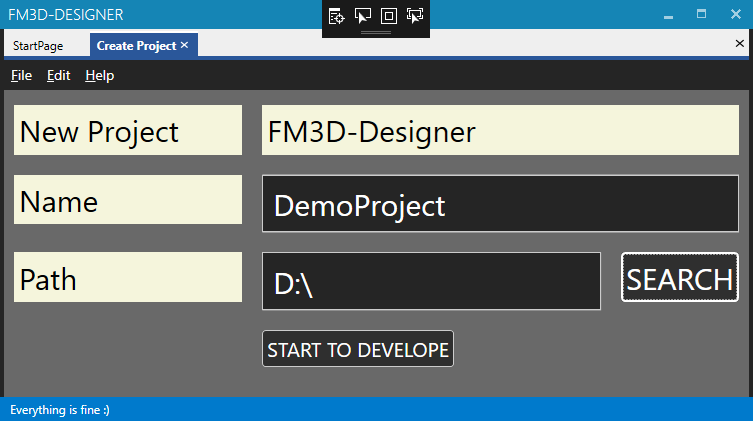
\includegraphics[width=0.5\textwidth]{04verwendung/Designer/00createproject.PNG}.
		\caption{Der Dialog um ein neues Projekt zu erstellen}\label{createprojekt}
	\end{center}
\end{figure}

\subsection{Altes Projekt laden}
\label{projektladen}
Falls Sie nun ein Projekt erstellt haben und es laden wollen, drücken Sie auf die Schaltfläche \textit{Load} rechts neben der Textbox. Es öffnet sich nun ein Explorer-Dialog in dem Sie nun eine \textit{.fmproj} Datei auswählen können. Wenn Sie nun eine Solche ausgewählt haben, drücken Sie auf \textit{Start}. Sie werden nun auf den Haupt-Arbeitsplatz des FM3D-Designers weitergeleitet.
Der Pfad des letzten geladenen Projektes kann durch den ContextMenü Punkt \textit{Last Project} in die Pfadleiste geladen und kann sofort geöffnet werden.

\subsection{Hauptarbeitsplatz}
Wenn sie nun in das Main-Layout (Siehe \cref{mainlayout}) gelangt sind befindet sich rechts ein File-Browser (Siehe \cref{filebrowser}). In diesem werden ihnen nun drei Ordner angezeigt. In diesen können Sie nun beliebig viele Entities und voraussichtlich\todo[inline]{wurk or nut wurk?} Ressourcen in das Projekt laden. Öffnen Sie nun ein Entity um verschiedene Komponente hinzuzufügen.
Auch können Sie Textdateien mit jeder beliebigen Endung zum Projekt hinzufügen.
Die Exportierten Ressourcen müssen Sie manuell in das Cpp Projekt einbinden.
Wenn Sie weitere Ordner in das Projekt einfügen wollen, speichern sie zunächst das Projekt ab und schließen Sie den FM3D-Designer. Gehen Sie dann in ihren Dateiexplorer, öffnen sie den Projektpfad und erstellen Sie an der beliebigen Stelle ein Verzeichnis. Laden Sie das Projekt neu über den Designer und klicken Sie mit der rechten Maustaste auf das Projekt-Item (Siehe \cref{item}). Ein \textit{ContextMenü} öffnet sich nun. Betätigen Sie den Schalter \textit{Include} und die Datei wird zum Projekt hinzugefügt.
\begin{figure}
	\begin{center}
		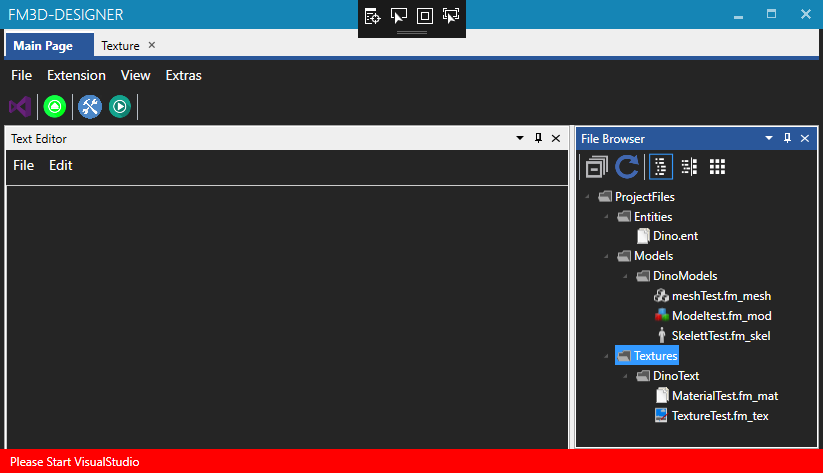
\includegraphics[width=0.5\textwidth]{04verwendung/Designer/01workstation.PNG}
		\caption{Der Haupt-Arbeitsplatz des FM3D-Designers}\label{arbeitsplatz}
	\end{center}
\end{figure}

\subsection{Extension}
Stellen Sie sicher, dass die FM3D-Extension installiert ist und starten sie darauf hin das VisualStudio-Projekt aus dem Designer. Klicken Sie, falls Sie es nicht schon getan haben, hierfür auf das Visual-Studio Icon im Designer. ([1] in \cref{extmen})
Bestätigen Sie die \textit{MessageBox} und warten Sie bis das Projekt geladen wurde.
Wenn es nun geladen wurde, überprüfen Sie nochmal ihre Entities im File-Browser. Falls alle ihren Vorstellungen übereinstimmen, gehen Sie nun auf den zweiten Schalter und betätigen Sie diesen. ([2] in \cref{extmen})
Nun werden die Entity-Preset Klassen in dem VisualStudio-Projekt generiert. Speichern Sie ihr Projekt anschließend.
Wenn sie ihr Spiel fertig Programmiert haben, so können Sie es über das Programm mit den zwei letzten Icons Debugen und Compilen ([3] und [4] in \cref{extmen}), falls Sie noch gerade im Designer beschäftigt sind. Diese Funktion ist optional.
\begin{figure}
	\begin{center}
		
\includegraphics[width=0.2\textwidth]{04verwendung/Designer/02ExtensionMenu.PNG}.
		\caption{Das Extension Menü}\label{extmen}
	\end{center}
\end{figure}
\section{Engine}
\label{verwendung_engine}
Wenn Sie die FM3D-Engine in Kombination mit dem FM3D-Designer verwenden, so wird Ihnen bei der Projekterstellung ein funktionsfähiges VisualStudio C++ Projekt generiert, welches in der VisualStudio-Solution \textit{GameProject.sln} zu finden ist.
Es wird Ihnen geraten, nichts an dem generierten Code zu ändern.
In der Datei \textit{"`presets.h"'} werden die Entity-Presets generiert, welche Sie im Designer erstellen können.
Sie können dem Projekt auch neue Dateien hinzufügen und unabhängig vom generierten Code programmieren. Weitere Dateien, welche ursprünglich nicht zu dem generierten Projekt gehört haben, sollten keinen Einfluss auf die Funktionalität des generierten Codes haben. Das Spiel an sich steht in der \textit{Main.cpp} Datei, welche im Projekt bereits vorhanden ist.

\subsection{Voreinstellungen}
Falls Sie die Engine in Kombination mit dem FM3D-Designer verwenden, so werden die Verzeichnisse automatisch eingebunden. Falls nicht, so müssen Sie Zunächst die Bibliotheken der FM3D-Engine, OpenGL, FreeImage, FreeType und Assimp in das Projekt manuell einbinden. Fügen Sie die Verzeichnisse in die zugehörige Option hinzu. Das ganze sollte so in ihren Einstellungen aussehen:
$$Configuration Properties->C/C++->Additional Include Directories$$\cref{includeinc}
$$Configuration Properties->Linker->Additional Include Directories$$
\cref{liblib}

\begin{figure}
	\begin{center}
		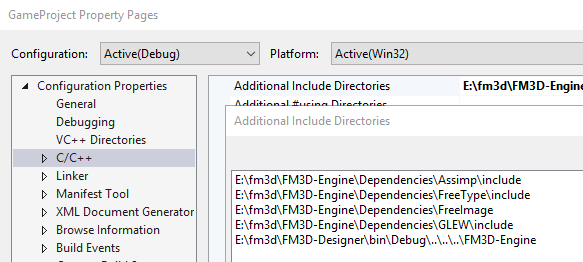
\includegraphics[width=\textwidth]{04verwendung/Engine/include.png}
		\caption{Include Verzeichnisse}\label{includeinc}
	\end{center}
\end{figure}

\begin{figure}
	\begin{center}
		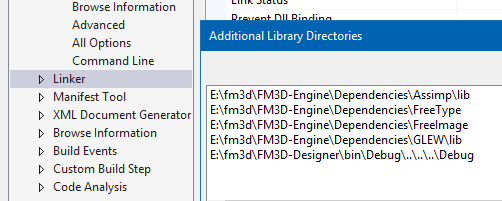
\includegraphics[width=\textwidth]{04verwendung/Engine/lib.png}
		\caption{Lib-Verzeichnisse}\label{liblib}
	\end{center}
\end{figure}

\subsection{Kamera}
Die Kamera ist in dem generierten Projekt bereits vorhanden. Ihnen wird empfohlen die Werte der Position, Rotation, Zoom usw. der Kamera im Bereich der \textit{Game-Logic} zu verändern. Auch dieser Bereich ist eindeutig mit Kommentaren kenntlich gemacht.
In dem erstellten Projekt existiert bereits ein Objekt der Klasse \textit{Camera}. Die \textit{Get}-Methoden geben eine Referenz zu dem jeweiligen Parameter der Kamera. Diese können somit sofort manipuliert werden. Als Beispiel:
\begin{lstlisting}{Cam}
// Create Camera Object
Camera camera(Vector3f(0.3f,0.4f,0.0f));
// Positionattribute Manipulation
camera.GetPosition().x += 0.5f;
camera.GetPosition().y -= 0.1f;
\end{lstlisting}
Für weitere Infos über die Syntax der Kamera wird empfohlen, in der DoxyGen-Dokumentation die Klasse "`Camera"' nachzuschlagen.

\subsection{Entities}
Erstellen Sie zunächst die Entities an der eindeutig kommentierten Stelle \textit{"'Create Entities here"`}. Erstellen Sie beliebig viele Preset-Objekte Ihrer erstellten Entity-Preset-Klassen. Sie können nun bei jedem beliebigen Objekt "`Preset-Einstellungen"' tätigen, in dem Sie dem Entity-Preset-Objekt Standardwerte zuweisen. Gehen wir davon aus, es gäbe ein Entitypreset Namens BaumPreset. Diesem wurde mittels Designer das RenderableComponent hinzugefügt.
\begin{lstlisting}{Entity}
BaumPreset baumpreset1;
\end{lstlisting}
Um nun dem Preset-Objekt ein Standartmodel zuzuweisen, verwendet man die folgende Syntax:

Erstellen wir zunächst ein Referenz-Objekt vom Typ Model.
\begin{lstlisting}{Entity}
Model* baummodel;
\end{lstlisting}
Um nun ein Model zu laden, wird die Klasse \textit{ExternFileManager} wie folgt verwendet:
\begin{lstlisting}{Entity}
ExternFileManager::
ReadModelFile("res/baum.dae", rendersystem, &baummodel, false, true);
\end{lstlisting}
Dies sagt nun Folgendes aus:
wir übergeben den Dateipfad "`res/baum.dae"' und ein Objekt des Render-Systems, in dem dann das Model gerendert werden soll. Daraufhin wird eine Adresse zu dem Objekt der Klasse \textit{Model} übergeben, in der das Model gespeichert wird. Der darauffolgende boolesche Wert gibt an, ob Instancing verwendet werden soll und der folgende, ob das Modell animierbar sein soll. Sie können nun dem Objekt Baum dieses Standartmodel zuweisen. Dies geschieht wie folgt:
\begin{lstlisting}{Entity}
baumpreset1.SetModel(&baummodel);
\end{lstlisting}
Initialisieren Sie nun einen Entity-Pointer (Klasse: \textit{EntityPtr}) und erstellen Sie das Entity in der bereits initialisierten \textit{EntityCollection} namens \textit{scene}. Als Beispiel:
\begin{lstlisting}{Entity}
EntityCollection scene;
EntityPtr baum = scene.CreateEntity();
\end{lstlisting}
Ein Objekt der Klasse \textbf{EntityCollection} beinhaltet alle Entities, die in dem Spiel verwendet werden. Jedoch können auch mehrere EntityCollection erstellt und verwendet werden.
Um die Presets auf einen Entity-Pointer und somit auf ein Entity in einer EntityCollection anzuwenden, wird die folgende Syntax verwendet:
\begin{lstlisting}{Entity}
baumpreset1.SetComponents(baum);
\end{lstlisting}
Nun wird dem EntityPointer alle Komponenten, mit den zuvor zugewiesenen Standartwerten, zugewiesen.

Wenn ein Entity das Komponent \textit{RenderableComponent} besitzt, so kann es in dem eindeutig kommentierten Abschnitt "`Submit objects here to renderer"' dem Renderer übergeben werden. Das heißt nun, dass das Model des Entities gerendert werden kann.
\begin{lstlisting}{Entity}
/// ##########################
  //
  //  Submit objects here to renderer!
  //
  renderer3D-Submit(baum.get());
/// ##########################
\end{lstlisting}
Bevor Sie den Entities die Modelle zuweisen, vergessen Sie nicht die Modelle in die Projektmappe von VisualStudio zu laden.

\subsection{Inputsystem}
\label{inputsystemver}
Hierfür wird die Klasse \textit{Input} verwendet. Möchte man nun Tasten abfragen, so muss man zunächst über das Fenster auf das Objekt der Klasse Input zugreifen. 
Nun kann eine Methode aus dieser Klasse verwendet werden.
Möchten Sie nun abfragen, ob z.B. die Taste F5 auf der Tastatur gedrückt wurde, so schreiben Sie dies so in den Code:
\begin{lstlisting}{Input}
win->GetInput().CheckKey(KEY_F5);
\end{lstlisting}
Möchten Sie nun überprüfen, ob die Linke Maustaste gedrückt wurde, so tun Sie dies folgendermaßen:
\begin{lstlisting}{Input}
win->GetInput().CheckMouse(MOUSE_LEFT);
\end{lstlisting}

Möchte man nun die Position des letzten Klicks der linken Maustaste ermitteln, benutzt man diese Methode:
\begin{lstlisting}{Input}
win->GetInput().GetLastposClick(MOUSE_LEFT);
\end{lstlisting}
Diese gibt einen zweidimensionalen Vektor vom Typ Float zurück, welcher die Position vom letzten Klick der Maus mit einer bestimmten Maustaste beschreibt. 
Die folgende Methode gibt Daten in Form eines zweidimensionalen Vektors mit der aktuellen Position der Maus zurück:
\begin{lstlisting}{Input}
win->GetInput().GetLastposInst();
\end{lstlisting}

Alle Tasten der Tastatur und Maus können über Makros angesprochen werden. Auch können Sie die ASCII-Codes der einzelnen Tasten verwenden. Die Makros, welche die Tasten der Tastatur beschreiben, starten mit \textit{"`KEY\_"'}. Die Makros, die für die Maus verwendet werden, starten mit \textit{"`MAUS\_"'}.
(Für weitere Informationen: Siehe DoxyGen Dokumentation)
\chapter{Resumé}

\section{Verbesserungsfähiges}
 Wie jedes Entwicklerteam hatten auch wir einige, nicht wenige Schwierigkeiten bei der Entwicklung unserer Software. Die wichtigsten Fehler und verbesserbaren Punkte haben wir hier dokumentiert.

\subsection{Software}
Der ursprüngliche Grund, warum wir den Designer entwickeln wollten, war das räumliche Darstellen von dreidimensional-renderbaren Entities und verschiedener Szenen vor dem Export in ein C++ Projekt. Handhaben wollten wir es ähnlich wie bei WPF: Eine Designer-Ansicht sollte die Übersicht und Optionen auf Entities liefern, welche mit einem Szenen-Editor editierbar wäre. Diese Ansicht sollte dem Nutzer die Ausgangslage des Spieles anzeigen.
Der Szenen-Editor sollte dem Nutzer ermöglichen, verschiedene Entity-Presets (siehe: \cref{entitysystem}) in eine Szene zu setzen. Die Szene würde dann mit XML- und Designer-spezifischen Skripten beschrieben und später wie Entities via Pipe (siehe\cref{pipe}) per Extension in Code umgewandelt werden.
Der Nutzer der Engine könnte dadurch selbständig ein komplett funktionsfähiges Programm generieren, ohne selbst programmieren zu müssen.
Wenn man nun einen solchen Skript-gesteuerten Szenen-Editor implementieren will, so müsste man auch einen komplexeren Text-Editor mit mehreren Funktionen implementieren. Er sollte an die Befehle für Skripte und XML angepasst werden und über automatische Wortvervollständigung für Befehle verfügen. Der Code müsste direkt bei der Eingabe auf Richtigkeit geprüft und Fehler sollten dem Nutzer angezeigt werden.
Um dem Nutzer ein besseres Spiel-Entwicklungserlebnis zu garantieren, könnte man den Entity-Editor in andockbare Fenster umlagern. So wäre es dem Nutzer möglich verschiedene Entities parallel zu bearbeiten.
Vieles der geplanten Ziele mussten aus Zeitmangel heraus gekürzt werden. (Grund: Siehe \cref{kleinanfangen})

\subsection{Team und Workflow}
\subsubsection{Planung}
Uns wurde schon relativ früh bewusst, dass die Planung bei einem größeren Projekt das A und O ist. Die Arbeitsschritte müssen am Anfang klar definiert sein, sodass man die Arbeit zum einen aufteilen und zum anderen planmäßig in einer festen Zeit fertigstellen kann. Bei unserem Projekt war die Planung gegen Anfang recht ausgefeilt, doch zählt nicht nur die Planung am Anfang des Projektes, sondern auch die Planung und Strukturierung während das Projekt am Laufen ist und die Kommunikation \ref{kommunikation} währenddessen. Es kam des öfteren vor, dass während der Entwicklung des Programmes bessere und effizientere Lösungsvorschläge in Frage kamen, als ursprünglich geplant war. Dies hatte oft auch eine Umstrukturierung des Projektes zur Folge. Als Beispiel nehme man das Entity-System(Siehe: \ref{entitysystem}). Zu Anfang wollten wir die ganzen Objekte aus Klassen erstellen, doch erwies sich dies als ungeeignet, da sonst verschiedene Objekte nur schwer miteinander interagieren könnten und außerdem müsste man jede Klasse einzeln definieren, was sehr viel Zeit beansprucht. 
Als wir das Entity-System nun eingeführt hatten, mussten wir natürlich das komplette Projekt dem Entity-System anpassen. Dort hatten wir einen Planungsdefizit.
                                                                                      
\subsubsection{Kommunikation}
\label{kommunikation}
Kommunikation ist das \textbf{wichtigste} bei einem komplexeren Projekt, bei dem mehrere Personen involviert sind. Um einen ununterbrochenen Arbeitsfluss zu garantieren, muss auch eine flüssige, detaillierte und verständliche Kommunikation vorhanden sein um Missverständnisse zu verhindern. Man muss immer bedenken, dass Mitarbeiter nicht in den Kopf anderer schauen können. So muss man seine Mitarbeiter immer über den eigenen Arbeitsfortschritt am laufenden halten.

\subsubsection{Klein anfangen}
\label{kleinanfangen}
Eines unserer größten Probleme war die Unterschätzung der von uns benötigten Zeit und die Überschätzung von uns selbst. So kam es, dass wir uns zu viele Funktionen überlegt hatten, die wir in unsere Lernleistung verarbeiten wollten, welche wir später aber des Zeitdruckes wegen wieder herausstreichen mussten. 
Wir haben uns des öfteren an mehreren Teilen des Programmes gleichzeitig aufgehalten. Dies hatte zwar zum einen den Vorteil, dass man immer am Arbeiten war und man so durch kleinere Erfolgserlebnisse die Motivation am Arbeiten nicht verlieren konnte. Dennoch hatte es den großen Nachteil, dass so wichtige Teile und Funktionen eines Programmes immer weiter bis zum Ende aufgeschoben wurden. Anstatt sich sofort diesen wichtigen Grundfunktionen zu widmen, steckten wir die Zeit so in Nebenfunktionen, die nicht essentiell wichtig für das Programm waren.
So wurde uns im Laufe des Projektes klar, dass es besser ist, mit einem kleiner konzipierten Programm anzufangen, bei dem die Grundfunktionen alle vollständig funktionsfähig sind und erst später, wenn das Grundgerüst und die Grundfunktionen eines Programmes stehen, man es ausbauen und verbessern kann. 

\section{Haben wir unser Ziel erreicht?}
Auch wenn viele der Funktionen, die wir uns zusätzlich vorgenommen hatten, der Zeit wegen aus dem Programm gefallen sind, haben wir dennoch unser Ziel erreicht. Wir haben uns vorgenommen eine Engine zu entwickeln, die dem Nutzer das Programmieren von Spielen erleichtert. Zudem wollten wir Tools entwickeln, die das Arbeiten mit der Engine vereinfachen und die Funktionen zur Unterstützung bieten.
Genau dies haben wir auch erreicht:
Wir haben eine funktionsfähige Engine "`\textit{from Scratch}"' geschaffen, mit der man ein komplettes Spiel, aber auch andere 3D-GUI-lastige Anwendungen programmieren kann. Zudem haben wir ein sehr nützliches Tool für die Programm-Entwicklung entwickelt, welches dem Entwickler eine Menge Code-Schreibarbeit abnimmt. 

\section{Was haben wir gelernt?}
Rückblickend können wir sagen, dass wir eine Menge durch diese besondere Lernleistung gelernt und auch verinnerlicht haben. Dies reicht von theoretischem bis hin zu praktischem Wissen. 
Die analytische Auseinandersetzung verschiedener Game-Engines (siehe \cref{engines}) und das Einlesen in Fachbücher zu diesem Thema hat uns die Tür in die Spiele- und Engine-Entwicklung geöffnet. Um nun 3D-Grafiken darzustellen mussten wir uns mit dem OpenGL Syntax(siehe \cref{opengl}) sowie Projektions- und Licht- Berechnungen (siehe \cref{rendering}) auseinander setzen.
Die Entwicklung des FM3D-Designers hat uns tiefe Einblicke in den C-Sharp Syntax ermöglicht. So konnten wir uns eine weitere Programmiersprache aneignen. Für das Projekte- und Dateien- Speichern, so wie es in unserem Designer geschieht, mussten wir uns den Umgang mit XML-Dateien (siehe \cref{extensiblemarkuplanguage}) und den dazugehörigen Bibliotheken aneignen.  Auch wurde unser Umgang mit dem C++ Syntax gefestigt. Zudem haben wir gelernt, wie man eine Extension für VisualStudio entwickelt und mit ihr kommunizieren kann.

\appendix
\chapter{Anhang}

\begin{acronym}
	\chapter*{Abkürzungsverzeichnis}
	\addcontentsline{SLERP}{chapter}{Abkürzungsverzeichnis}
	\acro{CLR} {Common Language Runtime}
	\acro{CPU} {Central Processing Unit}
	\acro{FBO} {Framebuffer Object}
	\acro{FM3D}{Flying Mind Engine}
	\acro{GPU} {Graphics Processing Unit}
	\acro{IBO} {Index Buffer Object}
	\acro{MVVM}{ModelView ViewModel}
	\acro{PBR} {Physically Based Rendering}
	\acro{VBO} {Vertex Buffer Object}
	\acro{VAO} {Vertex Array Object}
	\acro{WPF}	{Windows Presentation Foundation}
	\acro{XAML}{Extensible Application Markup Language}
	\acro{XML} {Extensible Markup Language}
	\acro{SLERP} {Spherical Linear Interpolation}
\end{acronym}

% Literaturverzeichnis
\bibliography{06anhang/literatur}

\end{document} %Process exited with error(s)